\documentclass[a4paper,10pt, titlepage, twoside]{article}

\usepackage{graphicx, verbatimbox}
\usepackage[nottoc,numbib, section]{tocbibind}
\usepackage{braket}
\usepackage{amsmath}
\usepackage{amssymb}
\usepackage{wrapfig}
\usepackage[left=1in, right=1in]{geometry}
\usepackage{fancyhdr}
\usepackage[ddmmyyyy]{datetime}
\usepackage{float}
\usepackage{tikz}
\usepackage{subcaption}
\usepackage{hyperref}
\hypersetup{
    colorlinks=true,
    linktoc=all,
    linkcolor=blue,
}

\newcommand{\Mod}[1]{\ (\mathrm{mod}\ #1)}

\pagestyle{fancy}
\fancyhf{}
\fancyhead[LE, RO]{42807671 - psycjw}

\begin{document}
\begin{titlepage}
	\centering
	
\includegraphics{uonlogo}\par
	\vfill
	{\huge Christopher J. Wright \par}
	\vfill
	{\huge \textbf{ID:} 42807671\par}
	{\huge \textbf{Supervisor:} Prof. Thorsten Altenkirch\par}
	{\huge \textbf{Module:} G53IDS\par}
	\vfill
	{\huge 2018/19}
\end{titlepage}
\shipout\null
\thispagestyle{empty}
\begin{titlepage}
	\centering
	
\includegraphics{uonlogo}	
	\vfill
	{\scshape\large G53IDS Dissertation \par}
	{\scshape\LARGE Quantum Computing in Haskell \par}
	\vfill
	{\large Submitted April 2019, in partial fulfilment of the conditions for the award of the degree BSc Computer Science \par}
	\vfill
	{\large \textbf{Author:} 42807671, Christopher J Wright, psycjw \par}
	{\large \textbf{Supervisor:} Prof. Thorsten Altenkirch, psztxa \par}
	\vfill
	{\large School of Computer Science \par University of Nottingham}
	\vfill
	{I hereby declare that this dissertation is all my own work, except as indicated in the text.\par}
	\vfill
	\begin{flushleft}
		{\large \textbf{Signature} \par}
		\vfill
		{\large \textbf{Date} \hspace{2cm} \today\par}
	\end{flushleft}
\end{titlepage}
\shipout\null

\fancyhead[RE, LO]{ABSTRACT}
\section*{Abstract}
Quantum computing is growing daily as new quantum computers are created, and new research is done. There are already many desirable uses of quantum computing, such as factoring integers in $O(log N)$ \cite{shor} and searching unsorted databases in $O(\sqrt{N})$ \cite{grover}. There are even quantum games being created, such as Quantum Battleships \cite{qships}. \par
As the field expands, more people will find interest in the field and attempt to learn and pursue a career concerning quantum computers, and so suitable learning and experimental platforms need to be present to help this happen. This is the main inspiration for this project; create a stable up-to-date platform for users to run quantum computations on a classical computer via quantum simulation, while also improving my own understanding and experience of the subject for the future.\par
This dissertation explains the basics of quantum computing, and provides possible methods for the implementation of certain quantum algorithms on a classical computer using Haskell, with a quantum-computation simulating package called QIO \cite{qio}. This package already includes structures necessary for quantum computations, such as the qubit and unitary functions, however does not work on the latest Haskell update (v8.4.3) and lacks complex quantum algorithms. Therefore, the package is first updated, and then two quantum algorithms are implemented. Following this, a quantum circuit builder is designed and implemented in the package, allowing users to create and test quantum circuits using a intuitive GUI.\par
Each part of the project, namely the implementation of two algorithms, Grover's algorithm and Shor's algorithm, and the quantum circuit builder, is completely separate and functions independantly. Due to this, I split the project up into three parts. Each part is designed, implemented, tested and evaluated before moving to the next part - avoiding confusion between parts and ensuring one part is complete before attempting the next.
\newpage

\fancyhead[RE, LO]{\leftmark}
\tableofcontents
\clearpage
\fancyfoot[CE,CO]{\thepage}

\setcounter{page}{1}
\section{Introduction to Quantum Computing}
\subsection{Brief History}
The idea of a quantum computer was first introduced in a talk in 1981 by Nobel prize-winning physicist Richard P. Feynman. In his talk, reproduced in the \textit{International Journal of Theoretical Physics} in 1982 \cite{feynman}, he proposed that it would be impossible to simulate a quantum system on a classical computer efficiently. At the same time, physicist Paul Benioff demonstrated that quantum mechanical systems can model classical Turing machines \cite{benioff}, and created the first recognizable theoretical framework for a quantum computer. \par
This resulted in David Deutsch's creation of the first universal quantum computer \cite{deutsch}. This computer could do things that a universal Turing machine cannot, such as generate truly random numbers, and simulate finite physical systems. \par
Over time, quantum algorithms have been developed which solve problems faster and more efficiently than classical algorithms can, demonstrating the main use for quantum computers. The main examples of such algorithms would be the Deutsch-Jozsa algorithm  \cite{deutsch-jozsa}, Shor's algorithm \cite{shor} and Grover's algorithm \cite{grover}.

\subsection{QIO}
QIO is a Haskell package built by Alexander S. Green and Prof. Thorsten Altenkirch \cite{qio}, which allows users to simulate a quantum computer on their own classical computer. Typical quantum operations are built up of unitary (reversible) functions under a monoid \texttt{U}, and can then be run using a monad \texttt{QIO} and the function \texttt{applyU}. This \texttt{QIO} monad also has functions \texttt{mkQbit} and \texttt{measQbit}, which can be used to create a new qubit and measure an existing qubit respectively.\par
This leads to an intuitive platform which can be used to create quantum computations, and then run/simulate them with 2 very simple functions \texttt{run :: QIO a -> IO a}  and \texttt{sim :: QIO a -> Prob a}, where \texttt{run} is used to execute a quantum computation and return the value of qubits measured based on their probabilities and a pseudorandom number generator. The \texttt{sim} function is similar, however after executing a quantum computation, it returns the probability distribution for the qubits measured, showing the possible states and their probabilities when measured.\par
Throughout this dissertation, this package is frequently used to help introduce and teach quantum computing, providing relevent code segments to improve clarity, and create programs which highlight certain features of quantum computations.

\subsection{The Qubit}
A classical computer uses a bit to store data. This bit can only be in one of two states, 0 or 1. Strings of bits are then used to represent data and instructions, forming the basis of classical computation.\par
However, a quantum computer uses a quantum bit, known as a qubit. This qubit can simply be in the classical states 0 or 1, or in a superposition of both, i.e., be in both states at once. This means an operation performed on a qubit effectively acts on both 0 and 1 at the same time.\par
A qubit can be described by a linear combination of $\ket{0}$ and $\ket{1}$, 
$$\ket{\psi}=\alpha\ket{0} + \beta\ket{1},\quad \alpha,\beta \in \mathbb{C},\quad |\alpha^2| + |\beta^2| = 1$$
where $ |\alpha^2|$ represents the probability of measuring the $0$ state, and $|\beta^2|$ the $1$ state. Hence the normalization condition $|\alpha^2| + |\beta^2| = 1$. This condition also corresponds to the fact that $\ket{\psi}$ is a unit vector in the complex vector space.\par
Measuring a qubit will collapse its wave function due to Born's rule \cite{born}. This means that, when measured, a qubit will collapse to be either $\ket{0}$ or $\ket{1}$. For example, if we take the qubit
$$\ket{+} = \frac{1}{\sqrt{2}}\ket{0} + \frac{1}{\sqrt{2}}\ket{1}$$
and measure it, the probability of getting $\ket{0}$ or $\ket{1}$ is $\frac{1}{2}$. We can therefore say that the qubit $\ket{+}$ is in an equal superposition.\par
In QIO, a qubit is referred to as a \texttt{Qbit}. One can be created simply using the \texttt{mkQbit :: Bool -> QIO Qbit} function mentioned above, and is created based on the boolean value passed in. The function \texttt{measQbit :: Qbit -> QIO Bool} can then later be used to measure the state of the qubit passed in.
\begin{verbatim}
make2qubits :: QIO (Bool, Bool)
make2qubits = do
    q0 <- mkQbit False -- This will create a qubit, q0, in the state |0>
    q1 <- mkQbit True -- This will create a qubit, q1, in the state |1>
    b0 <- measQbit q0 -- This will measure the qubit q0, returning False
    b1 <- measQbit q1 -- This will measure the qubit q1, returning True
    return (b0, b1) -- Returns (False, True)
\end{verbatim}
Qubit base states can also be represented as vectors, with $\ket{0} = 
\begin{bmatrix}
	1 \\ 0
\end{bmatrix}$
and $\ket{1} = 
\begin{bmatrix}
	0 \\ 1
\end{bmatrix}$.
The qubit $\ket{\psi}$ above can be rewritten, introducing a multiplier known as the global phase, making the coefficient for $\ket{0}$ (i.e., $\alpha$) real and non-negative. For example, the state $\frac{-i}{\sqrt{2}}\ket{0} + \frac{i}{\sqrt{2}}\ket{1}$ is the same as  $\frac{1}{\sqrt{2}}\ket{0} + \frac{-1}{\sqrt{2}}\ket{1}$ with a global phase of $-i$. This global phase does not affect the amplitudes of the states, and so doesn't change the qubit's value when measured.\par
This qubit state $\ket{\psi}=\alpha'\ket{0} + \beta'\ket{1}$  can now be written in the form
$$\ket{\psi} = \cos(\frac{\theta}{2})\ket{0} + e^{i\phi}\sin(\frac{\theta}{2})\ket{1},\qquad \theta = 2\cos^{-1}(\alpha'), \quad \phi = \Im(\ln(\frac{\beta'}{\sin(\frac{\theta}{2})}),$$
$$0 \leq \theta \leq \pi,\quad 0 \leq \phi \leq 2\pi$$
From this, it is easy to see that a qubit can be represented geometrically using the angles $\theta$ and $\phi$, on what is known as the Bloch sphere.

\subsection{The Bloch Sphere}
The Bloch sphere, named after physicist Felix Bloch, is a geometrical representation of a two-state quantum mechanical system (e.g. a qubit). As shown above, a qubit's coefficients can be expressed in terms of 2 angles, $\theta$ and $\phi$. This makes it extremely easy to see what happens when operations are performed on qubits, and it is clear that a qubit pointing to a point above the origin has a higher $\ket{0}$ amplitude than $\ket{1}$, and vice versa.\par
\begin{figure}[H]
	\centering
	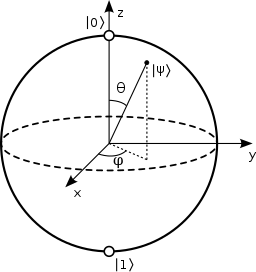
\includegraphics[width=0.25\textwidth]{blochsphere}
	\caption{A Qubit represented geometrically on the Bloch Sphere}
\end{figure}
We can calculate the angle $\theta$ using QIO's underlying structure and the \texttt{sim} function. The angle $\phi$ cannot be calculated in this way, as we use the probabilities for each state for the calculation.\par
The \texttt{sim} function returns a value of type \texttt{Prob a}, where \texttt{a} is given by the quantum computation it is applied to (i.e. applying \texttt{sim} to a function of type \texttt{QIO Bool}, will return a value of type \texttt{Prob Bool}). This \texttt{Prob} type is simply a wrapper around vectors given by real probabilities, defined in the \texttt{Qio.hs} file:
\begin{verbatim}
data Prob a = Prob {unProb :: Vec RR a}
\end{verbatim}
where \texttt{RR} is simply a \texttt{Double} value, and \texttt{Vec} is a wrapper around a list of pairs, defined in the \texttt{Vec.hs} file:
\begin{verbatim}
newtype Vec x a = Vec {unVec :: [(a,x)]} deriving Show
\end{verbatim}
From this, it is easy to see that
\begin{verbatim}
Prob Bool = Prob {unProb :: Vec RR Bool} 
          = Prob {unProb :: Vec {unVec :: [(Bool, Double)]}}
\end{verbatim}
Now, we can extract the probabilities for qubits, and calculate $\theta$.
\begin{verbatim}
quantum :: QIO Bool
quantum = do
    q <- mkQbit True
    measQbit q
    
theta :: QIO Bool -> Double
theta c = 2 * (acos alpha)
    where
        ps = unVec $ unProb $ sim c
        alpha = sqrt $ snd $ last ps
\end{verbatim}
The function \texttt{quantum} can be changed to perform any operation on the qubit, and as long as the function's type does not change, then \texttt{theta quantum} will always return $\theta$ for the qubit measured. E.g.
\begin{verbatim}
quantum :: QIO Bool        -> theta quantum = 3.141592653589793
quantum = do
    q <- mkQbit True
    measQbit q

quantum :: QIO Bool        -> theta quantum = 0.0
quantum = do
    q <- mkQbit False
    measQbit q

quantum :: QIO Bool        -> theta quantum = 1.5707963267948966
quantum = do
    q <- mkQbit False
    applyU (uhad q)
    measQbit q
\end{verbatim}

\subsection{Decoherence}
Put simply, decoherence is the loss of coherence. This basically means that the quantum state described by a system is no longer in superposition, and leads to a collapse of the wave function. If this occurs during a computation, all information stored in qubits is lost, and the computation needs to be restarted. Decoherence can occur naturally after a certain amount of time as the system will be entangled with its environment \cite{decoherence}, and is the main problem quantum computing faces.

\subsection{Basic Operations}
\subsubsection{1-Qubit Gates}
A 1-qubit gate can be thought of as a rotation about the Bloch sphere, and as the state space of a qubit is continuous, there are an infinite amount of 1-qubit gates. Any complex unitary 2x2 matrix represents a 1-qubit gate, and there are 4 main 1-qubit gates: the Hadamard gate, and the 3 Pauli- gates. Note that all quantum gates must be unitary (i.e., is its own inverse).\par
As mentioned earlier in section 1.2, QIO uses a monoid \texttt{U} to form unitary functions. These functions are defined as 5 distinct forms, using recursion to create sequences of functions:
\begin{verbatim}
data U = UReturn
       | Rot Qbit Rotation U
       | Swap Qbit Qbit U
       | Cond Qbit (Bool -> U) U
       | Ulet Bool (Qbit -> U) U
\end{verbatim}
\texttt{UReturn} is simply an empty function, and will always be the last unitary in a sequence. For this section on 1-Qubit gates, the \texttt{Rot Qbit Rotation U} form is used. QIO defines all single qubit gates as rotations, where a \texttt{Rotation :: ((Bool, Bool) -> CC)} represents the 2x2 matrix of the gate. The \texttt{rot} function is then used to create a unitary function for a given \texttt{Rotation} and qubit.
\begin{verbatim}
rot :: Qbit -> Rotation -> U
rot x r = Rot x r UReturn
\end{verbatim}

\paragraph{The Hadamard Gate}
Named after French mathematician Jacques Hadamard, the Hadamard gate (also called the Hadamard rotation) takes the base states $\ket{0}$ and $\ket{1}$ into equal superpositions
$$\ket{0} \mapsto \frac{1}{\sqrt{2}}(\ket{0} + \ket{1}) = \ket{+}$$
$$\ket{1} \mapsto \frac{1}{\sqrt{2}}(\ket{0} - \ket{1}) = \ket{-}$$
and has the matrix $\frac{1}{\sqrt{2}} 
\begin{bmatrix}
	1 & 1 \\
	1 & -1 
\end{bmatrix} $.
It is equivalent to the combination of 2 rotations: $\pi$ about the Z-axis, followed by $\pi/2$ about the Y-axis.
\begin{figure}[H]
	\centering
	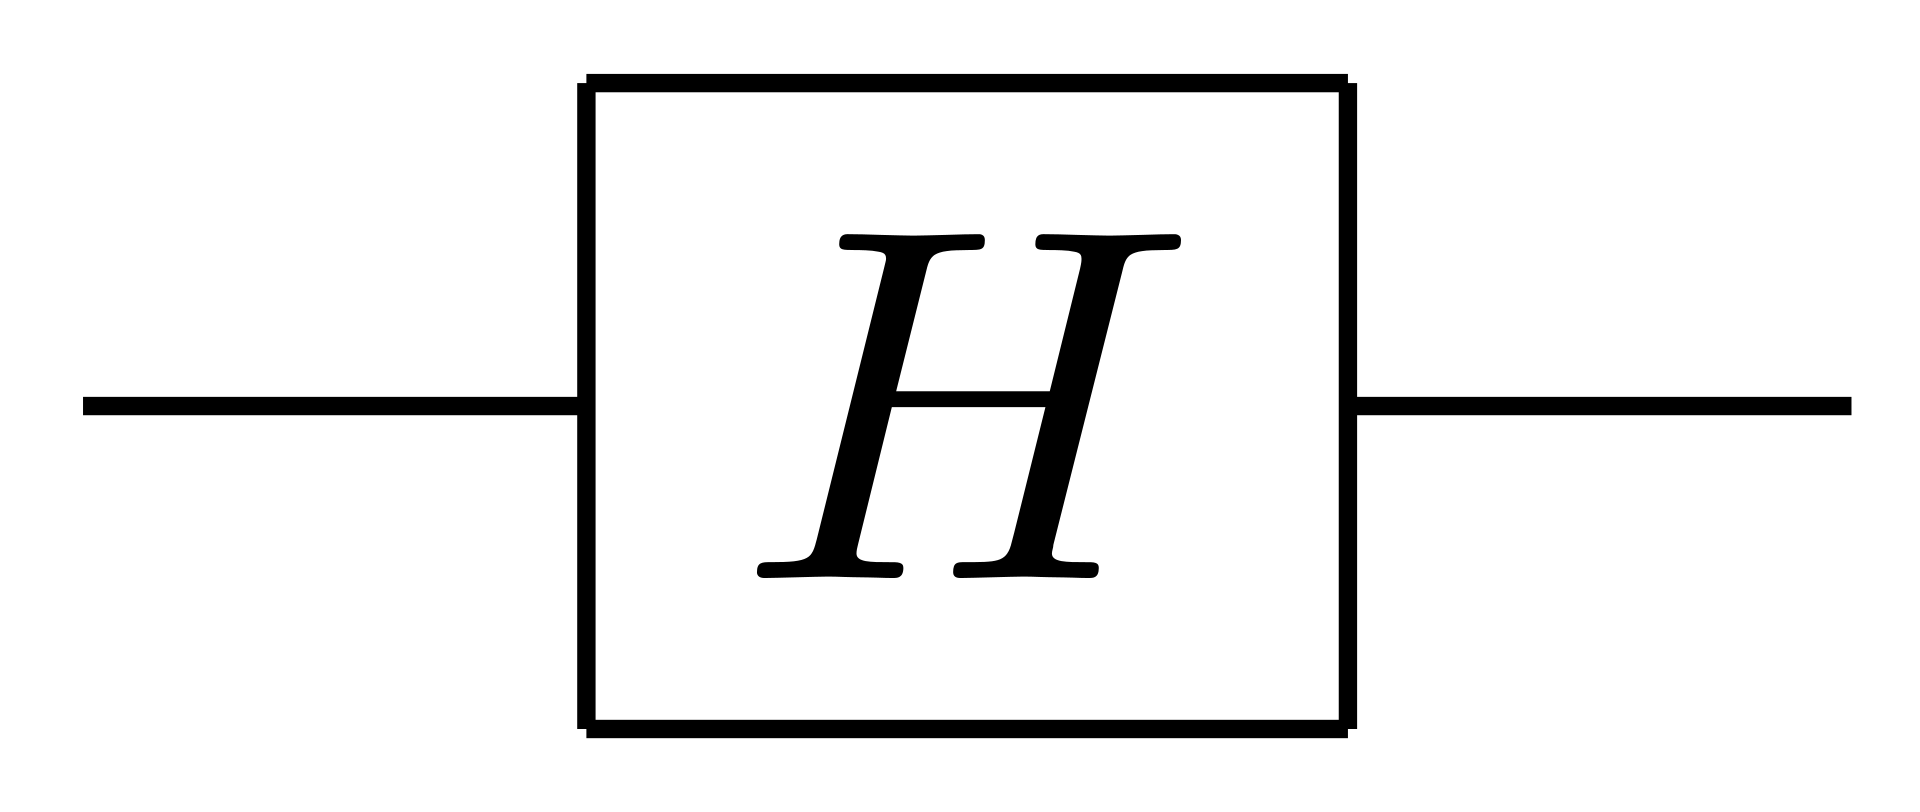
\includegraphics[width=0.25\textwidth]{hadamard}
	\caption{The Hadamard Gate}
\end{figure}
The gate matrix (i.e. \texttt{Rotation}) is given by \texttt{rhad} in the \texttt{QioSyn.hs} file, along with the unitary function \texttt{uhad} which can be used via the \texttt{applyU} function.
\begin{verbatim}
rhad :: Rotation
rhad (x,y) = if x && y then -h else h where h = (1/sqrt 2)

uhad :: Qbit -> U
uhad x = rot x rhad

applyHadamard :: QIO Bool
applyHadamard = do
    q <- mkQbit False
    applyU (uhad q)
    measQbit q
\end{verbatim}

\paragraph{The Pauli- Gates}
The Pauli- gates, created by Wolfgang Pauli, correspond to a rotation of $\pi$ about one of the 3 axis, and so there are 3 - Pauli-X, Pauli-Y and Pauli-Z (often abbreviated to X, Y and Z respectively). The Pauli-X gate is most common, as it is the equivalent of a classical NOT gate.

$$
X = 
\begin{bmatrix}
	0 & 1 \\
	1 & 0
\end{bmatrix},
\quad Y =
\begin{bmatrix}
	0 & -i \\
	i & 0
\end{bmatrix},
\quad Z =
\begin{bmatrix}
	1 & 0 \\
	0 & -1
\end{bmatrix}$$
\begin{figure}[H]
	\centering
	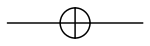
\includegraphics[width=0.25\textwidth]{not}
	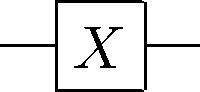
\includegraphics[width=0.18\textwidth]{paulix}
	\caption{The 2 representations of the Pauli-X (NOT) Gate}
\end{figure}
The Pauli-X gate is defined in QIO using the \texttt{rnot Rotation} and the unitary \texttt{unot}. However, these gates can be created simply by first creating the corresponding \texttt{Rotation} matrix, and then using the \texttt{rot} function similar to how the Hadamard gate is defined.

\begin{verbatim}
rX :: Rotation                          uX :: Qbit -> U
rX (x,y) = if x==y then 0 else 1        uX q = rot q rX

rY :: Rotation                          uY :: Qbit -> U
rY (False, True) = 0 :+ 1               uY q = rot q rY
rY (True, False) = 0 :+ (-1)
rY (_, _) = 0

rZ :: Rotation                          uZ :: Qbit -> U
rZ (False, False) = 1                   uZ q = rot q rZ
rZ (True, True) = -1
rZ (_, _) = 0
\end{verbatim}

\subsubsection{n-Qubit Gates}
Alongside the gates above, there are 3 other basic quantum gates; Controlled-X, SWAP and Toffoli, which are defined in QIO using the other 3 constructs for \texttt{U}.

\paragraph{The SWAP Gate}
This gate is extremely simply; it just swaps 2 qubits. In QIO, it is defined by the \texttt{swap} function.
\begin{verbatim}
swap :: Qbit -> Qbit -> U
swap x y = Swap x y UReturn
\end{verbatim}

\paragraph{The Controlled-X Gate}
The most common 2-qubit gate, it applies the Pauli-X gate (i.e., a NOT gate) on the second qubit if and only if the first qubit is $\ket{1}$. It is often called the Controlled-NOT or cNOT gate. Note that we can do the same with the other Pauli- gates, however this is rarely used.\par
The gate is defined using the \texttt{Cond Qbit (Bool -> U) U} unitary construct, and the function \texttt{cond} which creates the unitary (similar to the functions \texttt{rot} and \texttt{swap} above). Essentially, when given a qubit and a unitary function which takes in a boolean, the resulting unitary will apply the boolean function to the states the qubit can be in.\par
This is best demonstrated with an implementation for the cNOT gate. If the qubit is measured to be \texttt{True} (i.e. in the $\ket{1}$ state), then the resulting unitary is a NOT gate. Otherwise, nothing will be done and the resulting unitary is empty.
\begin{verbatim}
cond :: Qbit -> (Bool -> U) -> U
cond x br = Cond x br UReturn

cnot :: Qbit -> Qbit -> U
cnot qc qo = cond qc (\x -> if x then (unot qo) else mempty)
\end{verbatim}

\paragraph{The Toffoli Gate}
This gate acts on 3 qubits, and is often called the ccNOT gate. This is because it applies the Pauli-X gate on the third qubit if and only if the first two qubits are both $\ket{1}$. 
\begin{verbatim}
toffoli :: Qbit -> Qbit -> Qbit -> U
toffoli q1 q2 qo = cond q1 (\x -> if x then (cnot q2 qo) else mempty)
\end{verbatim}
\begin{figure}[H]
	\centering
	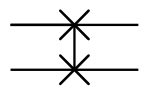
\includegraphics[width=0.25\textwidth]{swap}
	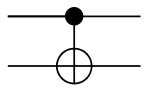
\includegraphics[width=0.25\textwidth]{cnot}
	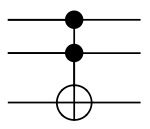
\includegraphics[width=0.25\textwidth]{toffoli}
	\caption{The SWAP gate (left), the Controlled-X (cNOT) gate (middle), and the Toffoli gate (right)}
\end{figure}

\paragraph{The $C^n$-NOT Gate}
The idea behind the Toffoli gate above (multiple control qubits, and one output qubit) can be extended to any arbitrary amount, creating a $c^n$-NOT gate. From the definition of the Toffoli gate in QIO above, it is clear that we can define a gate in QIO which acts on a list of control qubits, and one output qubit.
\begin{verbatim}
cNnot :: [Qbit] -> U
cNnot [] = mempty
cNnot (q:qs) = cond q (\x -> if x then (cNnot qs) else mempty)
\end{verbatim}
However, this only works due to how QIO operates on qubits. On a quantum computer, a gate like this will require a sequence of toffoli gates and ancilla qubits. For example, the cccNOT gate requires an extra ancilla qubit:
\begin{verbatim}
cccNot :: Qbit -> Qbit -> Qbit -> Qbit -> Qbit -> U
cccNot q1 q2 q3 q4 qa = 
    toffoli q1 q2 qa <>
    toffoli q3 qa q4 <>
    toffoli q1 q2 qa
\end{verbatim}
\begin{figure}[H]
	\centering
	\theverbbox\qquad
	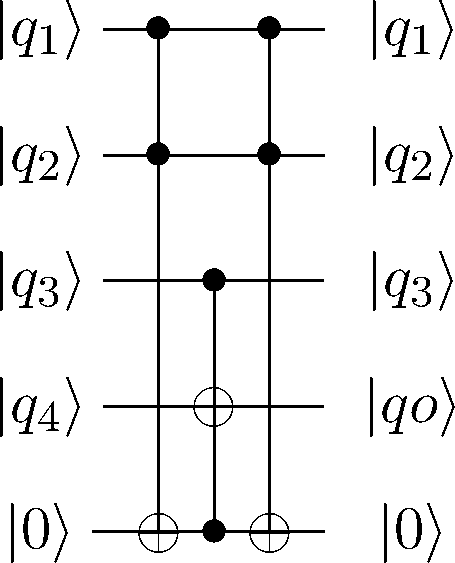
\includegraphics[width=0.25\textwidth]{cccnot}
	\caption{The cccNOT gate, made using toffoli gates and an ancilla qubit, where $\ket{qo} = \ket{q_4 \oplus (q_1 q_2 q_3)}$}
\end{figure}
When using ancilla qubits in QIO, we can use the unitary construct \texttt{Ulet} and the function \texttt{ulet}.
\begin{verbatim}
ulet :: Bool -> (Qbit -> U) -> U
ulet b ux = Ulet b ux UReturn
\end{verbatim}
This construct will create a qubit in the state given by the boolean, for use in the given unitary. We can now execute the cccNot gate defined above. The qubit \texttt{q4} will be set to $\ket{1}$ if and only if \texttt{q1, q2} and \texttt{q3} are all in the state $\ket{1}$.
\begin{verbatim}
doCccNOT :: QIO Bool
doCccNOT = do
    q1 <- mkQbit True
    q2 <- mkQbit True
    q3 <- mkQbit True
    q4 <- mkQbit False
    applyU (ulet False (cccNot q1 q2 q3 q4))
    measQbit q4
\end{verbatim}

\subsection{Entanglement}
Quantum entanglement is a phenomenon that occurs when the value of one qubit affects another, and forms a large part of many quantum algorithms. As mentioned above, when we measure a qubit it collapses to one of its base states. If another qubit depends on this measured qubit (e.g., via a cNOT gate), then it will also collapse to one of the base states. The 2 qubits are then said to be entangled. \par
Consider a circuit which starts with two qubits \textit{Alice} and \textit{Bob}, both starting in the state $\ket{0}$. We then apply the Hadamard gate to \textit{Alice}, converting \textit{Alice} into an equal superpositional state of the base states $\ket{+} = \frac{1}{\sqrt{2}}(\ket{0} + \ket{1})$, meaning there is a 50/50 chance of \textit{Alice} being 0/1 when measured. Next, we apply a cNOT gate to \textit{Alice} and \textit{Bob}, entangling the two qubits together. Therefore, if we measure \textit{Alice} to be $\ket{0}$, then \textit{Bob} will collapse to the state $\ket{0}$, and the same will occur for the state $\ket{1}$. As entanglement is non-local, \textit{Alice} and \textit{Bob} could be separated by any distance, and this will still occur.\par
This can be implemented in QIO using the \texttt{uhad} and \texttt{cnot} defined earlier. The function \texttt{entangle} below will create 2 qubits, \texttt{qa} and \texttt{qb}, and initialize them in the $\ket{0}$ state. We then apply the Hadamard gate to qa, changing its state to $\frac{1}{\sqrt{2}}(\ket{0} + \ket{1})$ and a controlled-X unitary function, concatenated simply with the mappend operator \texttt{<>}. When run using the \texttt{run} function, \texttt{[True, True]} or \texttt{[False, False]} will be returned due to the entanglement. The \texttt{sim} function will return \texttt{([True, True], 0.5), ([False, False], 0.5)}.\par
\begin{verbatim}
entangle :: QIO [Bool]
entangle = do
    qa <- mkQbit False
    qb <- mkQbit False
    applyU (uhad qa <> cnot qa qb)
    ba <- measQbit qa
    bb <- measQbit qb
    return [ba, bb]
\end{verbatim}

\subsection{The Bell States}
The two qubits shown above, \textit{Alice} and \textit{Bob}, together form a Bell state, named after physicist John S. Bell
$$\ket{\Psi_{00}} = \frac{1}{\sqrt{2}}\ket{00} + \frac{1}{\sqrt{2}}\ket{11} = \frac{1}{\sqrt{2}}(\ket{00} + \ket{11})$$
As evident from the equation, if one of the qubits is measured to be $\ket{0}$ or $\ket{1}$, then so is the other. There are 4 Bell states, where each state has 2 entangled qubits, and the measurement of one qubit collapses the state of the other.
$$\ket{\Psi_{00}} = \frac{1}{\sqrt{2}}(\ket{00} + \ket{11}) \quad \ket{\Psi_{01}} = \frac{1}{\sqrt{2}}(\ket{01} + \ket{10})$$
$$\ket{\Psi_{10}} = \frac{1}{\sqrt{2}}(\ket{00} - \ket{11}) \quad \ket{\Psi_{11}} = \frac{1}{\sqrt{2}}(\ket{01} - \ket{10})$$
Each Bell state is created using the same unitary operation, namely a Hadamard gate on the first qubit, and then a cNOT to the second qubit using the first qubit as the control bit, with the resulting Bell state determined by the original state of the 2 qubits.

\section{Motivations}
\subsection{Problems}
A quantum computer consists of multiple two-level quantum-mechanical systems, such as multiple electrons, with each electron represents a qubit. The spin of the electron determines the qubit state, with spin up representing $\ket{0}$ and spin down representing $\ket{1}$. The main problem faced here is decoherence \cite{decoherence2}. The overall system is extremely sensitive to interaction with the surroundings, such as magnetic fields affecting electrons, and must be isolated from its environment. The more qubits we have, the harder it is to maintain coherence.\par
Due to the difficulties of creating a quantum computer, we need to be able to simulate one on a classical computer. This simulation will not be as efficient as a quantum computer, and so its main use is the testing and creation of quantum algorithms, alongside teaching quantum computing. This means there is a high demand in quantum computing simulators, hence the need for projects like this.

\subsection{Simulators}
As mentioned above, creating a stable and effective quantum computer is difficult, and so while new ways of implementation are being researched, we can use quantum simulators to create, test and teach quantum computing. As quantum computing grows even larger, simulators need to be available to people in order to help them learn about quantum computations and programs. More quantum simulators across different programming languages will supply a wider range of programmers the ability to practice quantum computing on their own computer, as well as offer different methods of implementing a quantum simulator.\par
This project aims to add to this group of quantum simulators, offering an up-to-date and reliable Haskell package which enables users to create and run quantum programs. On top of this, they will be able to run quantum algorithms over their own data sets, increasing the teaching ability of the project.

\section{Related Work}
\subsection{IBM Q}
The IBM Q Experience is an online platform \cite{ibmqexperience} - found easily with a Google search "ibm q" - which gives its users access to a set of prototype quantum processors. Users can create quantum circuits or programs via a graphical or textual interface, and then either run these quantum operations on an actual quantum computer, or simulate them classically.\par
It was launched by IBM in 2016 \cite{ibmlaunch}, and started with a 5 qubit quantum processor and matching simulator, alongside a small set of two-qubit operations. Over time, the platform has evolved into a strong stable quantum platform, with the addition of more 2-qubit operations, a simulator over a maximum of 20 qubits and limited beta access to a 16 qubit quantum processor. IBM also released a python-based quantum computing framework, QISKit \cite{qiskit}, allowing users to simulate a quantum computer offline, or run quantum programs on the real IBM quantum processors online.

\subsubsection{Evaluation}
In my opinion, the IBM Q Experience platform is great for all who wish to create quantum programs and just generally experiment with quantum computing. A colourful, intuitive graphical interface can be used to build quantum circuits and then run/simulated with ease - perfect for new users. This still works well for more advanced users, however the textual interface is more suited for advanced use. Complex quantum programs can be created instead of circuits, and the use of the QISKit framework enables users the option of creating and simulating quantum computations without the online platform. However, this does mean users must learn a new programming language, potentially alongside learning about quantum computations, creating quite a large knowledge gap to bridge. Yet this is somewhat diminished by the availability of two user guides, a Beginner's guide \cite{ibmqbeginner} and a Full guide \cite{ibmqfull}.\par
These guides successfully reduce the difficulty in learning the basics of quantum computing without confusing newcomers. The Beginner's guide briefly explains the qubit, and common single qubit gates. It then goes on to hint at some multi qubit gates, and explain the process of entanglement and how it can be used. The Full guide extends these sections, providing a greater depth of knowledge concerning the qubit, such as the Bloch sphere and decoherence, while going into more detail on single and multi qubit gates, with descriptions of quantum algorithms and some quantum error correction methods. More help is then available to users via a community forum \cite{ibmqforum} and in-depth QISKit tutorials \cite{ibmqiskit}, ensuring users can find solutions to any problems they are having.

\subsubsection{Key Points}
\begin{enumerate}
	\item Simple and effective graphical user interface, allowing the user to drag-and-drop quantum gates onto a circuit, with bright colours used to emphasize different gates.
	\item Basic textual interface, providing users with an interface they can use to build more complex quantum programs.
	\item Multiple user guides to help teach newcomers without confusing them, while still providing aid to more advanced users. 
	\item Emphasis placed on usability.
\end{enumerate}

\section{Project Description}
\subsection{Aim}
The aim of this project is to update and improve an out-of-date Quantum computing package in Haskell, QIO \cite{qio} - developed by Green and Altenkirch. This will result in an updated, stable package for Haskell v8.4.3, allowing users to simulate a quantum computer, and run various quantum algorithms. It will also provide the user a graphical interface to build and run quantum circuits. \par
This QIO Haskell package allows a user to create a quantum program, and then run or simulate it. By running, any qubits measured via a function \texttt{measQbit :: Qbit -> QIO Bool} will be collapsed into True or False based on their probability amplitudes and a pseudorandom number generator. However, the difference between this package and others is revealed when we simulate the program instead. Then, any qubits measured will be shown as their probabilities, including multiple qubits together. From this we can easily check the program for errors.\par
The package is currently not working in Haskell v8.4.3, and so first needs to be updated. The update will need to maintain the quantum aspects necessary for quantum computation, such as coherence and the no-cloning theorem, and still be able to run/simulate quantum programs inputted. \par
Following this, two quantum algorithms (Grover's and Shor's) will be implemented in the package, allowing users to run these algorithms on their own data. There is already an implementation of Shor's algorithm present in QIO, but this needs to be updated. Each implementation will be in a separate Haskell file, and be able to perform a quantum algorithm correctly over its inputs using the rest of the QIO package.\par
Finally, a quantum circuit builder/interpreter will be built. It will display a graphical interface, and allow the user to drag-and-drop quantum gates onto a circuit of any amount of qubits. It will then display the resulting amplitude(s) and/or value(s) of any of the qubits. This will be similar to the IBM Q Program specified above, only shall be run on a classical computer instead of a quantum one.

\subsection{Algorithms}
\subsubsection{Grover's algorithm}
In 1996, Lov K. Grover demonstrated an algorithm which could search a quantum mechanical database quickly \cite{grover}. This quantum algorithm is quadratically faster than the fastest classical variant, returning the index of the search item in $O(\sqrt{n})$, instead of the classical $O(n)$. It can also be generalized to find solutions to an unknown predicate function $f$ in the same time. This means that any problem which involves finding solutions to a boolean function can be solved using Grover's algorithm, and so it has a large variety of uses past searching databases, such as finding the mean and median of a set of numbers, or solving the collision problem in $O(n^{1/3})$\cite{collision} instead of the classical $\Theta (\sqrt n)$\par
The algorithm takes a function $f$, and after converting it into a unitary function, runs it over a set of qubits representing the data set to search. It then negates solution states in the solution set, and disperses them. This dispersion acts as an inversion around the mean amplitude, meaning the solution state is amplified due to the previous negation. After repeating this a number of times no greater than $\pi/4\sqrt{N}$ times, where $N$ is the amount of variables in the function, there is a high probability that the qubits, when measured, will give a solution to the function $f$.\par
This project aims to explore potential methods of implementating this algorithm in the QIO Haskell package, as well as demonstrate other ways of executing the algorithm.

\subsubsection{Shor's algorithm}
Before Grover's algorithm, there was Shor's algorithm for integer factorization. This quantum algorithm is used to find the factors of any integer $N$ in ~$O((log N)^3)$ \cite{shorcomplexity}. The algorithm specifically looks at the case of factorizing an integer $N = pq$, where $p$ and $q$ are both large primes. If an integer $b$ shares no factors with $N$ then $b^r = 1 \Mod N$ for some integer $r$, and the function $f(x) = b^x \Mod N$ is a periodic function of $x$ with period $r$. With the period $r$ known, if it is even we can calculate
$$x = b^{\frac{r}{2}} \Mod N$$
Following this, if $x + 1 \neq 0 \Mod N$ we can factorize the input. The probability of choosing a random $b$ which gives a period $r$ with these properties is $>50\%$ \cite{nsc}\textsuperscript{Shor's algorithm continued, page 27}.\par
After constructing a unitary function $U_{f(x)} = b^x \Mod N$, the algorithm applies it over an input state, leaving an equal superpositional state 
$$\frac{1}{\sqrt{2^n/2}}\sum_{x=0}^{2^n-1} \ket{x}_n \ket{b^x \Mod N}_{n_0}$$
$$n_0 =\log_2 N,\quad n = 2n_0$$
We can then measure the second register, which will give any value for $b^x mod N$, leaving the first register in an equal superposition over the values for $x$. The algorithm then applies the Quantum Fourier Transformation (QFT) to the first register and measures it, giving a value for $y$ where $y = 2^n/r$. Finally, we can check if $r$ is even and if $x + 1 \neq 0 \Mod N$ where $x = b^{r/2} \Mod N$, and if they are both true, then $N$ has factors $(x-1)$ and $(x+1)$. We can then find the greatest common denominators of both in $N$, corresponding to the 2 prime factors of $N$.

\section{The QIO Package}
\subsection{Underlying Structure}
QIO currently uses a HeapMap to store the states of the qubits in the system, and a Qbit type which just acts as an integer reference to this map. Unitary functions take the form of a monoid \texttt{Unitary}, and represent an operation on the HeapMap which may produce a new state. We can then restrict unitary functions to be in a few distinct forms, ensuring the functions are indeed unitary - a necessity for quantum computations. These forms are defined in a datatype \texttt{U} shown below.
\begin{verbatim}
data U = UReturn 
       | Rot Qbit Rotation U 
       | Swap Qbit Qbit U 
       | Cond Qbit (Bool -> U) U 
       | Ulet Bool (Qbit -> U) U
\end{verbatim}

Using recursion, this type dictates is what a unitary operation will be; a string of rotations, swaps, conds and lets, ending in a UReturn. From these 4 operations, we can build any unitary operation possible, and as \texttt{U} is also defined as a monoid, we can easily concatenate operations together. Following this, the package defines another datatype \texttt{QIO a} - the type of a quantum computation:
\begin{verbatim}
data QIO a = QReturn a 
           | MkQbit Bool (Qbit -> QIO a) 
           | ApplyU U (QIO a) 
           | Meas Qbit (Bool -> QIO a)
\end{verbatim}
This datatype enables us to create and measure Qbits, along with applying unitary operations to them.\par
From all this, we can build a quantum program which creates qubits in an initial base state (i.e., either $\ket{0}$ or $\ket{1}$), applies any amount of unitary functions to them, and then measures qubits. Now we need to let the user execute a quantum program on a simulated quantum system. To do this, QIO has 2 functions: \texttt{run :: QIO a $\to$ IO a} and \texttt{sim :: QIO a $\to$ Prob a}.\par
Run takes a quantum computation in the type defined above, and executes it on a simulated quantum system. When qubits are measured and returned in the computation, the function prints this state value to the console using the IO monad. The state value to return will originally be a quantum state, and so is made up of probability amplitudes. Therefore, the actual state to return will be chosen at random based on these probability amplitudes and a psuedorandom number generator.\par
Sim, however, is a bit different. It still takes a quantum computation and executes it, however it returns the actual probabilities of the possible states the qubits measured may be in. This makes testing quantum programs fairly simple, drastically increasing the usability of the project. 

\subsection{Updating QIO}
\subsubsection{Current Errors}
Currently, QIO cannot be installed on the latest Haskell version (v8.4.3). This is because the package depends on the Haskell base package version being $\geq 4.9 \text{ and} < 4.10$. After downloading the package, and manually changing this to allow any base package $\geq 4.9$, two errors are shown depicting what is incorrect with the current QIO structure.\par
\begin{verbatim}
QIO/QioSyn.hs:39:10: error:
        * No instance for (Semigroup U)
            arising from the superclasses of an instance declaration
        * In the instance declaration for `Monoid U'
...
QIO/QioSynAlt.hs:118:10: error:
        * No instance for (Semigroup U)
            arising from the superclasses of an instance declaration
        * In the instance declaration for `Monoid U'
\end{verbatim}

From the error messages presented, it is clear that a change to Monoids is causing errors. In the update to base-4.11.0.0, the Haskell Semigroup class was made a superclass of Monoid \cite{base411}. This means that a Semigroup instance for \texttt{U} needs to be defined, alongside the Monoid instance.\par
The current definition for \texttt{U} in QioSyn.hs is shown below
\begin{verbatim}
instance Monoid U where
        mempty = UReturn
        mappend UReturn u = u
        mappend (Rot x a u) u' = Rot x a (mappend u u')
        mappend (Swap x y u) u' = Swap x y (mappend u u')
        mappend (Cond x br u') u'' = Cond x br (mappend u' u'')
        mappend (Ulet b f u) u' = Ulet b f (mappend u u') 
\end{verbatim}
All that needs to be done to fix this is to include a Semigroup definition for \texttt{U} which defines the structure for executing multiple unitary functions, and then to define mempty and mappend for the Monoid instance.
\begin{verbatim}
instance Semigroup U where
        UReturn <> u
        (Rot x a u) <> u' = Rot x a (u <> u')
        (Swap x y u) <> u' = Swap x y (u <> u')
        (Cond x br u') <> u'' = Cond x br (u' <> u'')
        (Ulet b f u) <> u' = Ulet b f (u <> u')
        
instance Monoid U where
        mempty = UReturn
        mappend = (<>)
\end{verbatim}\par
After this, the alternate file QioSynAlt.hs needs to be updated also. The definition for \texttt{U} is very similar, however uses a non-recursive datatype in its definition.
\begin{verbatim}
instance Monoid U where
        mempty = Fx UReturn
        mappend (Fx UReturn) u = u
        mappend (Fx (Rot x a u)) u' = Fx $ Rot x a (mappend u u')
        mappend (Fx (Swap x y u)) u' = Fx $ Swap x y (mappend u u')
        mappend (Fx (Cond x br u')) u'' = Fx $ Cond x br (mappend u' u'')
        mappend (Fx (Ulet b f u)) u' = Fx $ Ulet b f (mappend u u') 
\end{verbatim}
The fix for this is very similar to before:
\begin{verbatim}
instance Semigroup U where
        (Fx UReturn) <> u = u
        (Fx (Rot x a u)) <> u' = Fx $ Rot x a (u <> u')
        (Fx (Swap x y u)) <> u' = Fx $ Swap x y (u <> u')
        (Fx (Cond x br u')) <> u'' = Fx $ Cond x br (u' <> u'')
        (Fx (Ulet b f u)) <> u' = Fx $ Ulet b f (u <> u') 
        
instance Monoid U where
        mempty = Fx UReturn
        mappend = (<>)
\end{verbatim}\par

\subsubsection{New Errors}
After updating the files, the package produces 2 new error messages when attempting to build, and the previous errors do not show. The same errors are occuring (lack of a Semigroup instance) but for different files, QioClass.hs and Qio.hs.
\begin{verbatim}
QIO/QioClass.hs:17:10: error:
        * No instance for (Semigroup UnitaryC)
            arising from the superclasses of an instance declaration
        * In the instance declaration for `Monoid UnitaryC'
...
QIO/Qio.hs:32:10: error:
        * No instance for (Semigroup Unitary)
            arising from the superclasses of an instance declaration
        * In the instance declaration for `Monoid Unitary'
\end{verbatim}
Therefore, the fixes are the same as before: create a definition for a Semigroup instance based on the Monoid instance, then define mempty and mappend in the Monoid definition.
\begin{verbatim}
QioClass.hs:
instance Semigroup UnitaryC where
         (U f) <> (U g) = U (\ fv h -> g fv (f fv h))
        
instance Monoid UnitaryC where
        mempty = U (\ fv bs -> bs)
        mappend = (<>)

Qio.hs:
instance Semigroup Unitary where
        (U f) <> (U g) = U (\ fv h -> unEmbed $ do h' <- Embed $ f fv h
                                                   h'' <- Embed $ g fv h'
                                                   return h'')
                                                
instance Monoid Unitary where
        mempty = U (\ fv h -> unEmbed $ return h)
        mappend = (<>)
\end{verbatim}

\subsubsection{Testing}
After updating QioClass.hs and Qio.hs, the package builds and installs successfully onto Haskell v8.4.3. \textit{Note: The package still installs and runs correctly on the newest version of Haskell, namely v8.6.3.} Running various quantum programs using the updated package gives correct results, and so the package still works as intended after being updated, and so all that is left to do is change the base dependancy of the package to $\geq 4.11$.

\section{Algorithms}
During the following two sections, the algorithms mentioned earlier will be explained in more detail, along with explanations of their implementations in Haskell using the QIO package. The algorithms are each broken down into parts, and each respective part of the implementation is described simultaneously in an effort to maximise understanding.

\subsection{Grover's Algorithm}
As stated earlier in section 4.2.1, Grover's algorithm can be used to search a quantum database in $O(\sqrt n)$, and can be extended to solve any blackbox boolean function. This extension reveals the numerous uses Grover's algorithm has, and so will be the main focus for implementation. Allowing the user to input a custom function will abstract them away from the algorithm's complexity, enabling simple testing over multiple use cases - hopefully improving understanding.\par
In order to find a solution to a blackbox function - which returns 1 for a solution input, and 0 otherwise - a classical computer must repeatedly apply the function to random integers in order to find the solution, and so is $O(N)$. However, a quantum computer can find a solution to the function after applying it no greater than $\pi/4\sqrt{N/s}$ times - where $N$ is the amount of variables in the function, and $s$ is the amount of solutions to the function - with a probability of success close to 1 when N is large. While the algorithm works for all functions which produce either 0 or 1 based on the input, it is often still thought as just an algorithm which searches through an unsorted database faster than any classical method.\par
Put simply, Grover's algorithm takes in a blackbox function, creates a superposition over all possible function inputs and then emphasizes states which are not solutions. After doing this roughly $\pi/4\sqrt{N/s}$ times, there is a high probability that a solution state is found. The algorithm can be split up into multiple explicit parts:
\begin{enumerate}
	\item \textbf{The Oracle} -  Creating a unitary function based on the blackbox function, and applying it to a set of qubits.
	\item \textbf{Diffusion} - Increasing the amplitude of solutional state(s).
	\item \textbf{Measurement} - Measuring specific qubits to get a solution.
\end{enumerate}
\par
\subsubsection{The Oracle}
The blackbox function $f$ returns 0 or 1 based on if the inputted value (i.e. an $n$-bit integer) $x$ is the solution $a$;
$$f(x) = 0, \quad x \neq a \qquad f(x) = 1, \quad x = a.$$
This function can be represented in the form of a unitary function $U_f$, which acts on an $n$-qubit register containing $x$, and a single qubit register containing the result $f(x)$.
$$U_f(\ket{x}_n\ket{y}) = \ket{x}_n\ket{y \oplus f(x)}$$
A simple example of this would be a unitary function which returns 1 when 0010 is inputted, and 0 otherwise:
\begin{figure}[H]
	\centering
	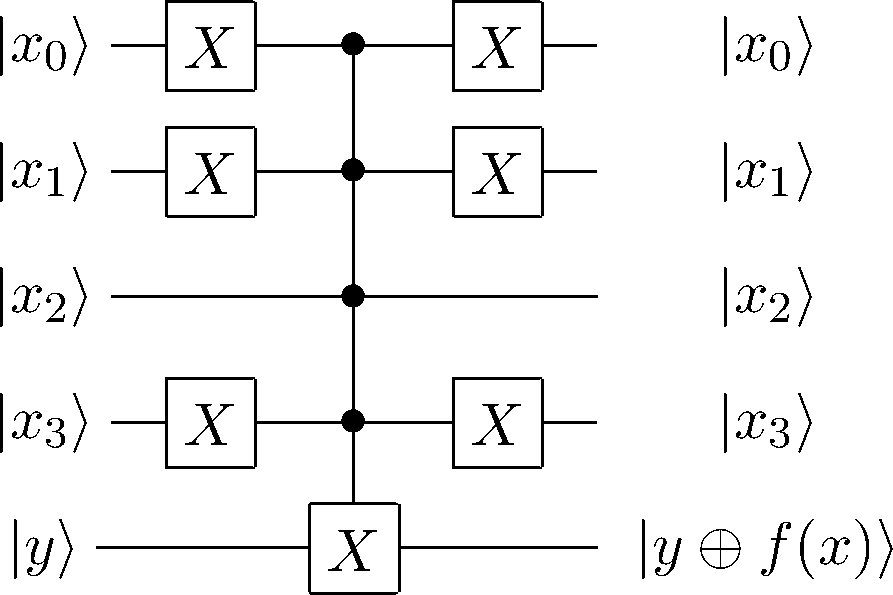
\includegraphics[width=0.25\textwidth]{oracle0010}
	\caption{A unitary function, setting the last qubit to 1 when 0010 is inputted, and 0 otherwise}
\end{figure}

This can be modified so that the overall state's sign is changed if $x = a$ by first setting the output qubit to $\ket{1}$ and applying the Hadamard gate to it before the application of $U_f$. So, the output qubit is in the state $H\ket{1} = \frac{1}{\sqrt{2}}(\ket{0} - \ket{1}) = \ket{-}$ before application, and after applying $U_f$ the overall state becomes
$$U_f(\ket{x} \oplus \ket{-}) = (-1)^{f(x)}\ket{x} \oplus \ket{-}$$
From this equation it is obvious that applying $U_f$ to the state is the same as doing nothing to the single output qubit, while applying a unitary transformation $V$ to the input register, where
\begin{equation}
	V\ket{x} = (-1)^{f(x)}\ket{x} = \begin{cases}
		\ket{x}, \quad x \neq a,\\
		-\ket{a}, \quad x = a.
	\end{cases}
\end{equation}

If we initially transform the n-qubit input register into a uniform superposition of all possible inputs, i.e.
$$\ket{\phi} = H^{\otimes n}\ket{0}_n = \frac{1}{2^{n/2}}\sum_{x=0}^{2^n-1}\ket{x}_n$$
Then, after applying $V$, the component of the state along $\ket{a}$ (i.e. the state we are looking for) will have a negative phase. The unitary $V$ can therefore be written as
$$V\ket{\Psi} = \ket{\Psi} - 2 \ket{a}\braket{a | \Psi} \qquad \therefore V = 1 - 2\ket{a}\bra{a}$$
\begin{figure}[H]
	\centering
	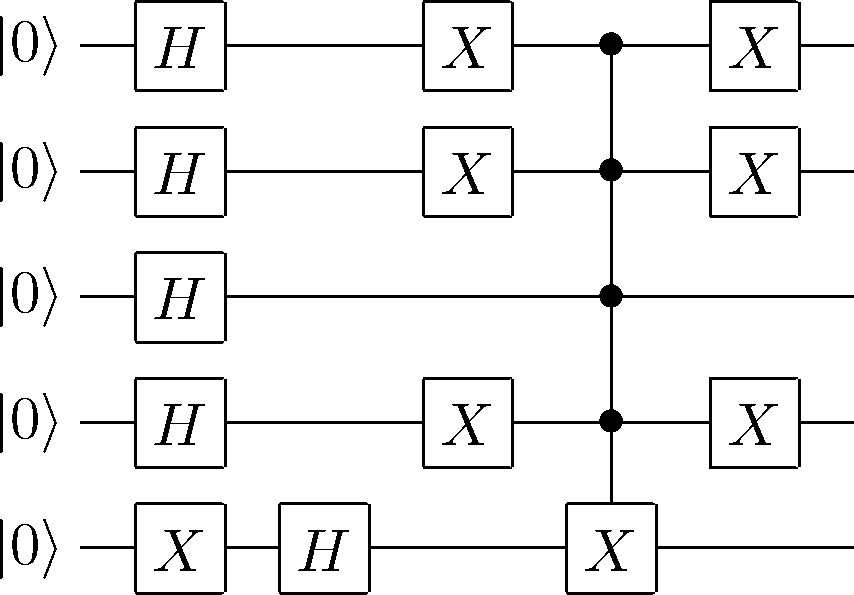
\includegraphics[width=0.25\textwidth]{oracle00102}
	\caption{Applying $V$ to an equal superposition of all possible inputs.}
\end{figure}

\paragraph{Implementation}
Before actually implementing the oracle used for Grover's algorithm in Haskell, it is useful to first define a few functions to work over lists of qubits - allowing easy expansion to custom oracles later on.
\begin{verbatim}
mkQbits :: Int -> Bool -> QIO [Qbit]}
mkQbits n b = mkQbits' n b []
  where
    mkQbits' 0 _ qs = return qs
    mkQbits' n b qs = do
      q <- mkQbit b
      mkQbits' (n-1) b (qs ++ [q])
\end{verbatim}

As you can see, \texttt{mkQbits} is a function which uses recursion to create a list of \texttt{n Qbit}s in the state given by \texttt{b}. This leads on to the creation of another function, \texttt{measQbits :: [Qbit] -> QIO [Bool]} which returns a list of boolean values representing the measurements of the inputted list of \texttt{Qbit}s. The only two remaining functions necessary pertain to applying unitary functions to lists of \texttt{Qbit}s. More specifically, we need a function which applies a single-qubit unitary operation to all qubits in a list, and another function which applies a single-qubit unitary operation to the last qubit in a list, conditional on the state of each other qubit in said list.
\begin{verbatim}
unitaryN :: (Qbit -> U) -> [Qbit] -> U
unitaryN _ []      = mempty
unitaryN uf (q:qs) = uf q <> unitaryN uf qs

condN :: (Qbit -> U) -> [Qbit] -> U
condN uf (q:[]) = uf q
condN uf (q:qs) = cond q (\x -> if x then (condN uf qs) else mempty)
\end{verbatim}

Now that these functions are created, initializing the qubits and applying the oracle is simple. First, we need to create $i$ qubits for each variable in the function and put them in the state $\ket +$, and then create $o$ qubits for each ``line'' in the function, each put in the state $\ket -$.

\begin{verbatim}
initialize :: Int -> Int -> QIO ([Qbit], [Qbit])
initialize i o = do
  qI <- mkQbits i False
  qO <- mkQbits o True
  applyU (unitaryN uhad (qI ++ qO))
  return (qI, qO)
\end{verbatim}

Now we need to create a function representing $V$, the oracle unitary. For now, this will be for the example above, searching for the state $\ket{110}$. 

\begin{verbatim}
oracle :: [Qbit] -> [Qbit] -> U
oracle qI qO =
  unot (qI!!2) <>
  condN unot (qI ++ [qO!!0]) <>
  unot (qI!!2)
\end{verbatim}

\subsubsection{Diffusion}
Grover's algorithm requires one more unitary $W$, which does not depend on the oracle function. This unitary transformation changes the sign of the component orthogonal to $\ket{\phi}$, i.e.
$$W = 2\ket{\phi}\bra{\phi} - 1$$
The unitary $-W$ works fine here, as the final state will only differ by an overall minus sign, if it differs at all. From $-W$, and the fact that the Hadamard gate is its own inverse, you can see that we need a gate which does nothing for all states apart from $\ket{00...00}$, which it multiplies by -1.
$$-W = 1 - 2\ket{\phi}\bra{\phi}, \qquad \ket{\phi} = H^{\otimes n}\ket{0}_n$$
$$\therefore -W = H^{\otimes n}(1 - 2\ket{00...00}\bra{00...00})H^{\otimes n}$$
\par
The Pauli-Z gate is the main gate to use here. This gate, with matrix 
$\begin{bmatrix}
	1 & 0 \\
	0 & -1
\end{bmatrix}$
, multiplies the state $\ket{11...11}$ by -1, and does nothing on all other states. From this, it is easy to see that if we applied a controlled Pauli-Z gate to the qubits, surrounded by $n$ Pauli-X gates, we get the unitary $-W$.
$$-W = H^{\otimes n} X^{\otimes n} (c^{n-1}Z) X^{\otimes n} H^{\otimes n}$$

\paragraph{Implementation} 
Implementing this is extremely simple using the functions created earlier, as shown below

\begin{verbatim}
diffuse :: [Qbit] -> U
diffuse qI =
  unitaryN uhad qI <>
  unitaryN unot qI <>
  condN (\q -> uphase q pi) qI <>
  unitaryN unot qI <>
  unitaryN uhad qI
\end{verbatim}

\subsubsection{Application \& Measurement}
All that is left now is to apply $WV$ repeatedly to the intital state $\ket{\phi}$ enough times for a solution state to be found. This is best described using simple geometry.\par

\begin{wrapfigure}{l}{0.55\textwidth}
\centering
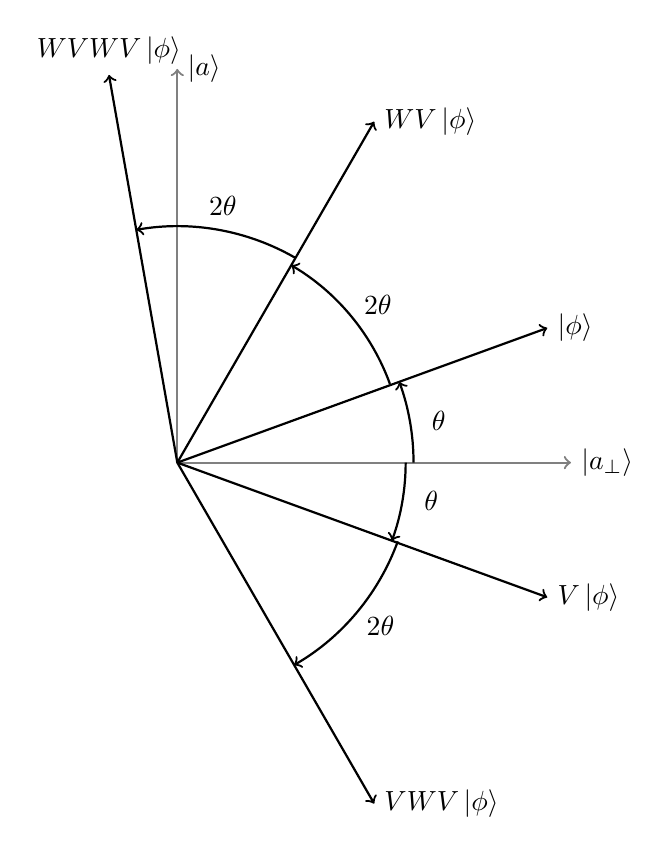
\begin{tikzpicture}
    \coordinate (origin) at (0,0);
    \draw[thick,gray,->] (origin) -- (5,0) node [black,right] {$\ket{a_\perp}$};
    \draw[thick,gray,->] (origin) -- (0,5) node [black,right] {$\ket{a}$};
    \draw[thick,black,->] (origin) -- (20:5) node [black,right] {$\ket{\phi}$};
    \draw[thick,black,->] (origin) -- (-20:5) node [black,right] {$V\ket{\phi}$};
    \draw[thick,black,->] (origin) -- (60:5) node [black,right] {$WV\ket{\phi}$};
    \draw[thick,black,->] (origin) -- (-60:5) node [black,right] {$VWV\ket{\phi}$};
    \draw[thick,black,->] (origin) -- (100:5) node [black,above] {$WVWV\ket{\phi}$};
    
    \draw[thick, black, ->] (3,0) arc (0:20:3) node [black,xshift=0.5cm,yshift=-0.5cm] {$\theta$};
    \draw[thick, black, ->] (2.9,0) arc (0:-20:2.9) node [black,xshift=0.5cm,yshift=0.5cm] {$\theta$};
    \draw[thick, black, ->] (2.7,1) arc (20:59.5:2.9) node [black,xshift=1.1cm,yshift=-0.5cm] {$2\theta$};
    \draw[thick, black, ->] (2.8,-1) arc (-20:-60:3) node [black,xshift=1.1cm,yshift=0.5cm] {$2\theta$};
    \draw[thick, black, ->] (1.5,2.6) arc (60:100:3) node [black,xshift=1.1cm,yshift=0.3cm] {$2\theta$};
\end{tikzpicture}
\end{wrapfigure}

The intial state $\ket{\phi}$ will contain one state $\ket{a}$ with amplitude $\frac{1}{2^{n/2}} = 1 / \sqrt{N}$, and so starts out at an angle $\theta$ from $\ket{a_\perp}$, where $\sin{\theta} = 1 / \sqrt{N}$.\par
The unitary $V$ negates the state $\ket{a}$ in $\ket{\phi}$, and so on the graph, it reflects $\ket{\phi}$ about the axis $\ket{a_\perp}$. Next, the unitary $W$ is applied which negates any state orthogonal to $\ket{\phi}$ (i.e. any negative state in $\ket{\phi}$, notably the state $\ket{a}$). Graphically, this means the unitary $W$ reflects about $\ket{\phi}$, and so when applied to $V\ket{\phi}$, it results in a state at an angle of $3\theta$ above $\ket{a_\perp}$. Therefore, each iteration (application of the unitary $V$ followed by $W$) rotates the qubits' state by $2\theta$ anti-clockwise, giving us a simple method to find out the amount of iterations, $i$, required. Note: when N is large, $\sin{\theta} \approx \theta$.
$$\theta + 2i\theta \approx \pi / 2  \qquad \sin{\theta} = 1 / \sqrt{N} \qquad \therefore \theta \approx 1 / \sqrt{N}$$ 
$$\therefore i \approx \frac{\pi - 2\theta}{4\theta} \approx \frac{\pi}{4} \sqrt{N}$$
\par
The amplitude of the state $\ket{a}$ over the qubits is given by the sine of the angle between the qubits and $\ket{a_\perp}$, and so the probability of measuring the solution from the qubits is equal to the square of this.

\paragraph{Example}
Say we want to search for $\ket{110}$ across a space of 8 (i.e. 3 qubits). The iterations required will therefore be $\approx \frac{\pi}{4} \sqrt{8} \approx 2$. The oracle function will perform a controlled-X gate on its output qubit if its inputs are in the state $\ket{110}$. Then, we need to diffuse the qubits using the unitary $W$ described above. After initializing the qubits, we must apply $V$, then $W$, and repeat this again to get a solution. 
\begin{figure}[H]
    \centering
    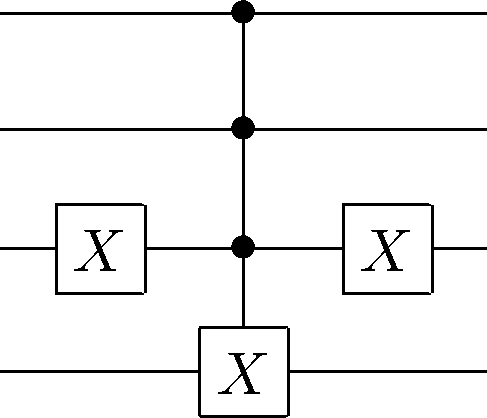
\includegraphics[width=0.25\textwidth]{grovers110V}
    \hspace{1cm}
    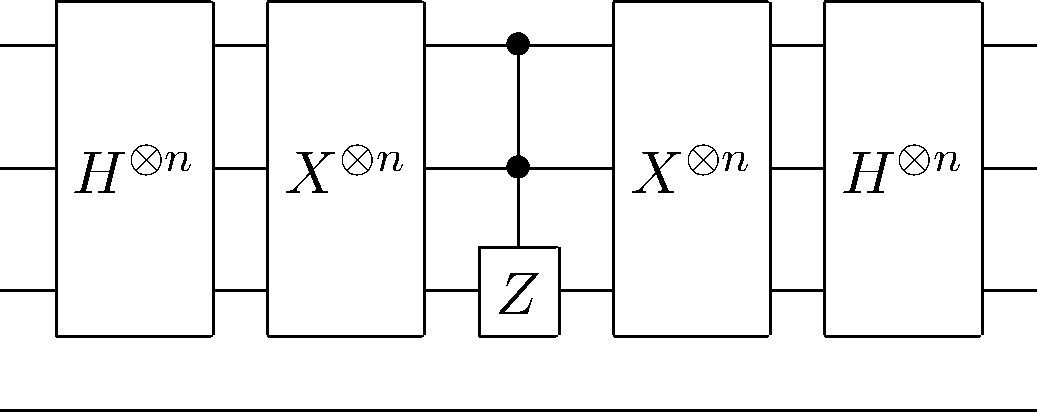
\includegraphics[width=0.5\textwidth]{grovers110W}
    \caption{The 2 unitaries $V$ (left) and $W$ (right) used to search for $\ket{110}$.}
\end{figure}
\begin{figure}[H]
    \centering
    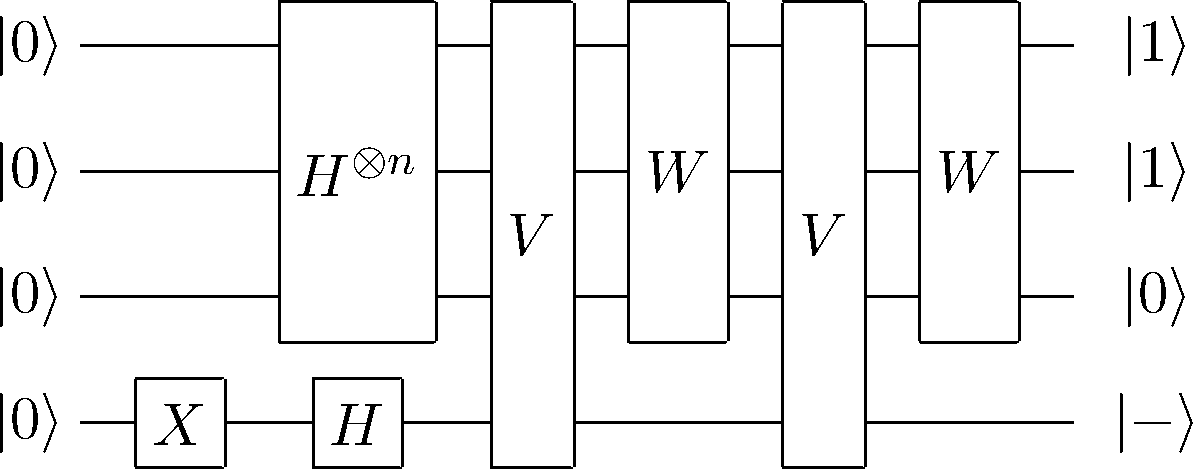
\includegraphics[width=0.5\textwidth]{grovers110}
    \caption{The circuit used to perform Grover's algorithm over 3 input qubits, with solution $\ket{110}$.}
\end{figure}

\paragraph{Implementation}
All that remains in the implementation is to combine the functions described above and apply them the correct amount of times (i.e. twice when searching for the state $\ket{110}$).

\begin{verbatim}
grover :: QIO [Bool]
grover = do
  (qI, qO) <- initialize 3 1
  let groverStep = oracle qI qO <> diffuse qI
  applyU (groverStep)
  applyU (groverStep)
  measQbits qI  
\end{verbatim}

\paragraph{Testing}
Testing this is relatively simple: simply \texttt{run} the \texttt{grover} function, check the result and then \texttt{sim} the function, checking the probability of expected results.\par
\begin{verbbox}
run grover -> [True, True, False]
sim grover -> [..., ([True, True, False], 0.9453125), ...]
\end{verbbox}

\begin{figure}[H]
    \centering
    \theverbbox \\
    with all other states having probability $7.812...e^{-3}$
\end{figure}

\subsubsection{Expansion to multiple solutions}
The algorithm above can also search for multiple solutions, the only thing that changes is the amount of iterations necessary. If there are $s$ solutions, then the amount of iterations required becomes $i \approx \frac{\pi}{4} \sqrt{\frac{N}{s}}$.\par

\subsubsection{Implementing a Custom Oracle}
In the example above, the oracle is searching for \texttt{True, True, False}, i.e. $x1 \land x2 \land \neg x3$. So, if the program takes in a function as a boolean predicate, it can create a unitary function representing the oracle using a list of the input variables in the predicate, and applying 2 NOT gates to negated variables.\par
The oracle can also search for multiple lines of predicates separated by OR operations; simply have a different output qubit for each line, so that solutions to every line will be negated, allowing easy usage for multiple solutions. For example, if the user wants to apply the algorithm over a function $f$, where
$$f(x_n) = (x1 \land x2 \land x3) \lor (\neg x1 \land x2 \land \neg x3)$$
then they can input\par
\begin{verbbox}
1 2 3
-1 2 -3
\end{verbbox}
\begin{figure}[H]
    \centering
    \theverbbox
\end{figure}

So the oracle function needs to be changed to take in a list of a list of \texttt{Int}s, i.e. \texttt{[[Int]]}, where each inner list represents a line of the function. From this, it will recursively apply the NOT gates over qubits referenced by negative integers, and apply controlled-X gates over the qubits referenced in each line to the output qubits, where each inner list is applied to its own unique output qubit.\par
\begin{verbatim}
oracle :: Int -> [[Int]] -> [Qbit] -> [Qbit] -> U
oracle _ [] _ _ = mempty
oracle c (p:ps) qI qO =
  unitaryN unot (unots p qI) <>
  condN unot (conds p qI ++ [q0!!c]) <>
  unitaryN unot (unots p qI) <>
  oracle (c+1) ps qI q0
  where
    unots p qI = map (\x -> qI!!((abs x)-1)) $ filter (< 0) p
    conds p qI = map (\x -> qI!!((abs x)-1)) p
\end{verbatim}

The program also needs to know how many solutions there are in order to iterate the application of $V$ and $W$ the correct amount of times, roughly equal to $\frac{\pi}{4}\sqrt{\frac{N}{s}}$. The application can then be done using the \texttt{foldr} function, folding with the \texttt{mappend} operator \texttt{<>}, starting from \texttt{mempty}.\par
The entry point to the algorithm will be using the \texttt{main} function in the code. This function, of type \texttt{IO ()}, will take in a custom function inputted in the form described above, and then run the algorithm over it. This can also be timed effectively using the \texttt{TimeIt} package \cite{timeit}.

\subsubsection{Testing}
In order to test this, the program needs to be changed slightly to \texttt{sim} the algorithm, and print out the probabilities. The above predicate $x1 \land x2 \land \neg x3$, inputted as \texttt{1 2 -3} returns the expected result:

\begin{verbbox}
[...,([True, True, False]), 0.9453125),...]
\end{verbbox}

\begin{figure}[H]
    \centering
    \theverbbox
    \\ with all other states having probability $7.812...e^{-3}$
\end{figure}

A more complicated predicate shown below also returns the correct result, indicating the implementation works correctly. 
$$(x1 \land \neg x2 \land x3 \land x4) \lor (x2 \land \neg x3 \land x4) \lor (x1 \land x2 \land x3)$$
\begin{center}
Solutions: $0101, 1011, 1101, 1110, 1111$\\
Output: \\\texttt{[([True, True, True, True], 0.1914...),\\ ([True, True, True, False], 0.1914...),\\ ([True, True, False, True], 0.1914...),\\...,\\ ([True, False, True, True], 0.1914...),\\...,\\ ([False, True, False, True], 0.1914...), \\...]} with all other states having probability $3.906...e^{-3}$
\end{center}

\subsubsection{An Improvement}
This algorithm can be altered to actually not use any ancilla qubits in QIO  (due to the way QIO executes multi-qubit gates) and use less gates, improving run time. The current implementation uses ancilla qubits to negate solution states in the input qubits. However, this can simply be done using a controlled Pauli-Z gate over the inputs, when the input qubits are initially in the state $\ket{-}$. After this, the diffusion is also simplified to become an inversion about the mean \cite{groverblog}; decrease the amplitude of non-solutional states about the mean amplitude while increasing the amplitude of solutional states. This can be achieved by $n-1$ Hadamard gates surrounding a $C^n$-NOT gate.\par

\begin{figure}[H]
    \centering
    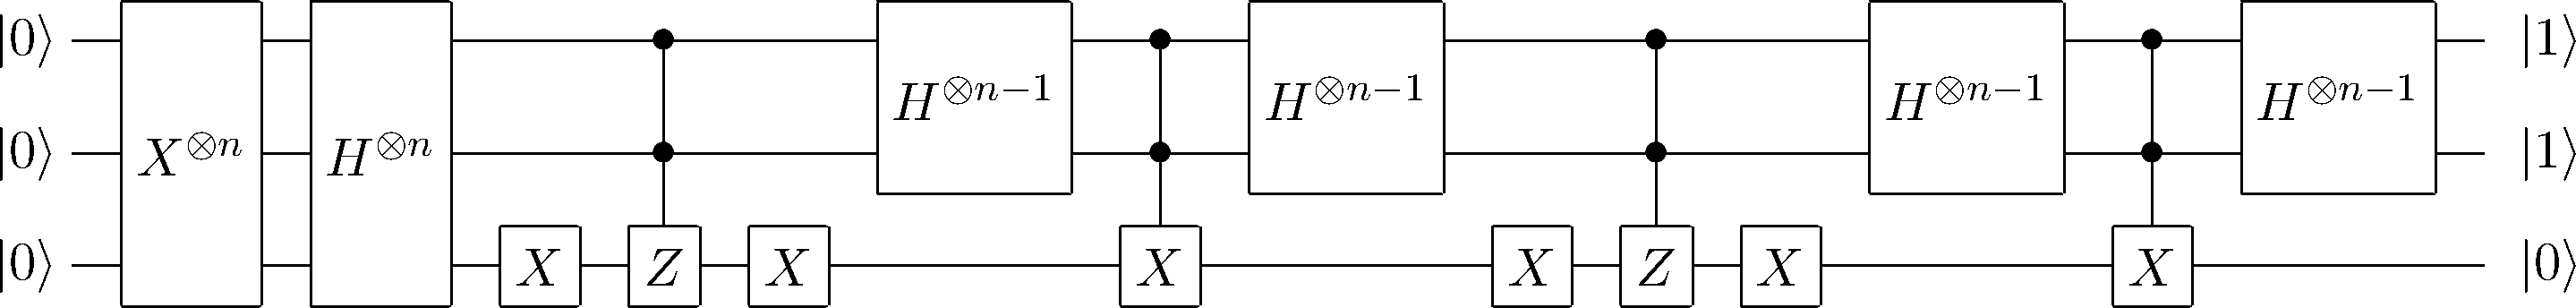
\includegraphics[width=\textwidth]{groverImp}
    \caption{Improved circuit for Grover's algorithm, searching for the state $\ket{110}$}
\end{figure}

In order to change the code to implement this, the \texttt{initialize}, \texttt{oracle} and \texttt{diffuse} functions need to be altered.

\subsubsection{Testing Solutions}
The current algorithm works well when solving a function with a known amount of solutions, and returns correct solutions with a high probability as shown. However, the implementation can be changed to measure whether or not the input qubits contain a solution at the end, This will enable the program to return definite, distinct solutions and find solutions to functions with an unknown amount of solutions.\par
By simply using ancilla qubits to test the state of input qubits with $C^n$-NOT gates, a final ancilla qubit will be in the state $\ket{1}$ if the input qubit's contain a solution.

\begin{figure}[H]
    \centering
    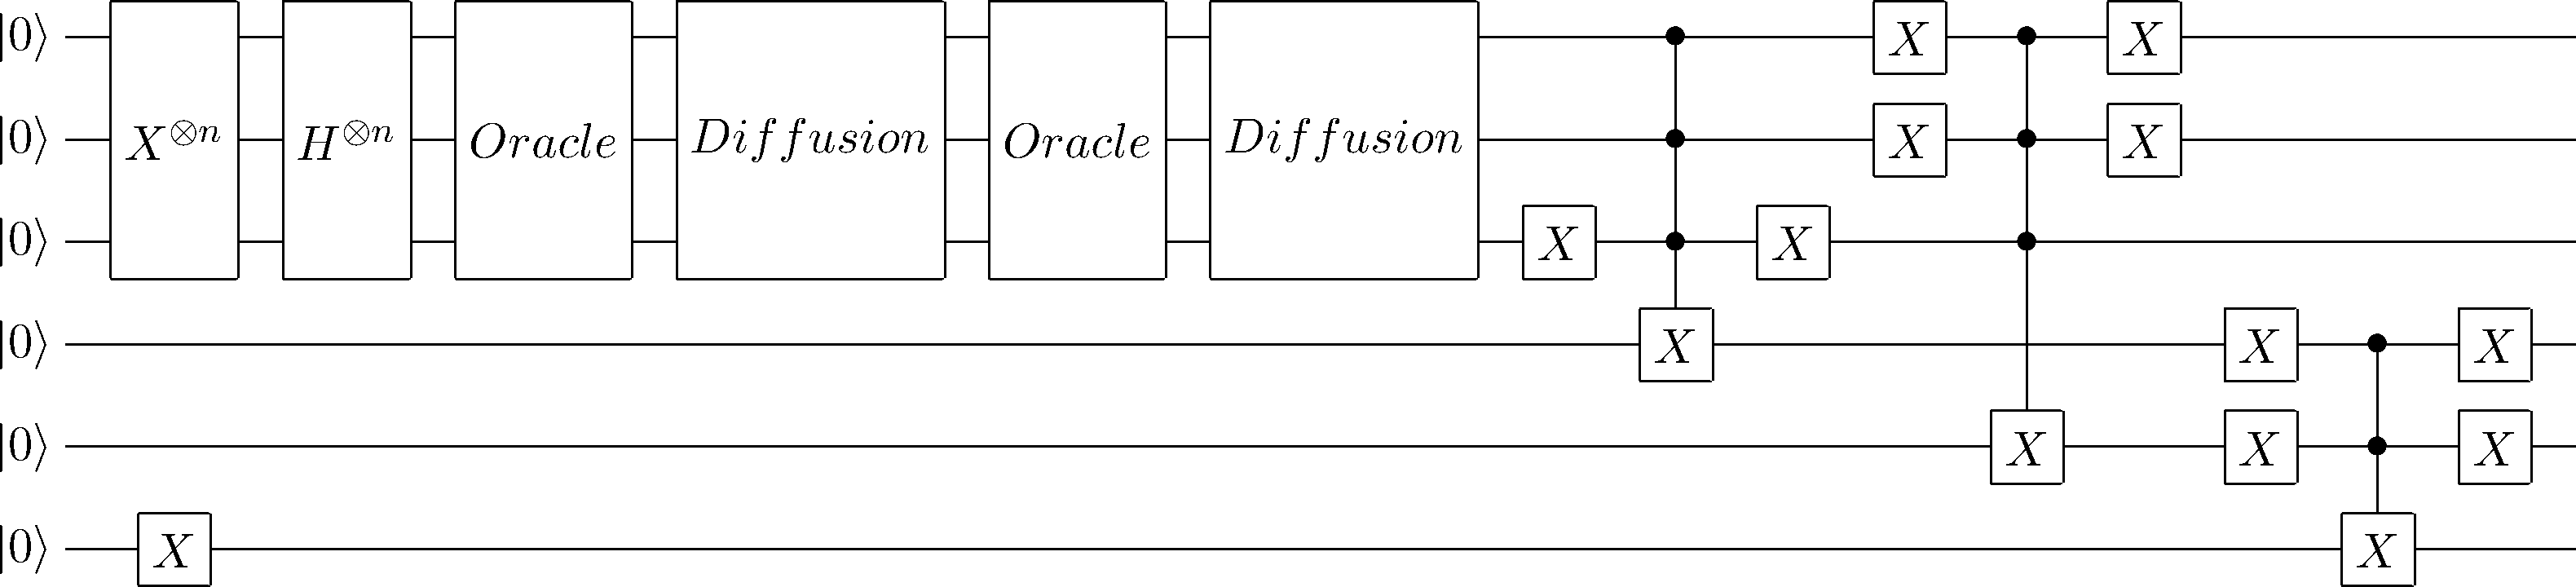
\includegraphics[width=\textwidth]{groverFinal}
    \caption{Improved circuit for Grover's algorithm, searching for the state $\ket{110}$ and $\ket{001}$, while also checking $n$ qubits for the solution.}
\end{figure}
The results of each line of the function (i.e. $x0 \land x1 \land \neg x2$ and $\neg x0 \land \neg x1 \land x2$) are saved into two separate qubits. Following this, a third ancilla qubit is set to $\ket{0}$ if both the two ancilla qubits are in the state $\ket{0}$, which would only occur when the input qubits do not contain a solution.

\paragraph{Implementation}
In order to implement this, the \texttt{initialize} function will need create the necessary ancilla qubits, all of which will be in the state $\ket 0$ except for the last, which will be in the state $\ket 1$. A new function needs to be created to apply the necessary $C^n$-NOT gates over the input qubits on distinct ancilla qubits, which will be applied after the algorithm has been executed. Finally, the program will measure the last ancilla qubit in the list, and return this with the measurements of the input qubits. The ancilla measurement can then be checked to determine if a solution was found, allowing easy looping to get multiple, unique and definite solutions. \par
This will also enable the algorithm to be used for functions with an unknown amount of solutions, as this requires multiple executions of the algorithm with differing amounts of iterations until a solution is found. In this case, the amount of iterations starts as $\frac{\pi}{4}\sqrt{N}$. If this does not result in a solution, the algorithm is executed again with $\frac{\pi}{4}\sqrt{\frac{N}{2}}$ iterations, and then $\frac{\pi}{4}\sqrt{\frac{N}{4}}$ iterations, and so on until a solution is found. The total amount of iterations required is still $O(\sqrt N)$ as shown below.
$$\frac{\pi}{4}\sqrt N \left(1 + \frac{1}{\sqrt 2} + \frac{1}{2} + \frac{1}{2\sqrt 2} + ...\right) = \frac{\pi}{4}\sqrt N \sum_{i=0}^{\infty}\frac{1}{2^i} = \frac{\pi}{4}\sqrt N (2 + \sqrt 2)$$

\subsubsection{Probability}
We can also print out the probability of finding the solution by running the \texttt{sim} function over a function which only measures the last ancilla qubit (which will only be measured to be True if the input qubits contain a solution).

\begin{verbatim}
probability :: Int -> Int -> [[Int]] -> IO ()
probability n i ps = putStrLn $ show $ sim $ probOfSolution
  where
    probOfSolution = do
      (qI, qA) <- initialize n ((length ps)+1)
      let groverStep = oracle ps qI <> diffuse qI
      applyU (foldr (<>) mempty (replicate i groverStep))
      applyU (testForSolution 0 ps qI qA)
      measQbit $ last qA
\end{verbatim}

\subsection{Shor's Algorithm}
As mentioned in section 4.1, there is already an implementation of Shor's algorithm in QIO, in the file \texttt{Shor.hs}. Therefore, this section will be dedicated to explaining the current implementation, and describing any potential improvements.\par
In section 4.2.2, it was stated that Shor's algorithm is for integer factorization. This is not exactly correct, as the algorithm actually finds the period of a function, which can then be expanded to factorize integers. Let $f$ be a function, periodic on addition, over integers, i.e.\par
$$f(x) \equiv f(y) \iff x = y + cr, \qquad c \in \mathbb{Z} $$
Classical algorithms for finding the period of such a function take a time which grows faster than any power of the number of bits of $r$. However, Shor's algorithm does this in a time which scales slightly faster than $n^3$ \cite{qscbook}\textsuperscript{Page 63}.\par
Put simply, the algorithm applies the function $f$ over two qubit registers. Measuring the second register, i.e. the register containing the results of $f(x)$, collapses the first into a superposition over all the values which give that measured value. Each of these values in the register will be separated by integer multiples of the period $r$. Finally, we apply an algorithm known as the quantum Fourier transformation, which extracts the value of the period $r$ from the register. We can then measure this register to obtain a value for the period. Similar to Grover's algorithm, it can be broken down into distinct parts:\par
\begin{enumerate}
    \item \textbf{Function Application} - Creating a unitary representation for the function $f$, and applying it to the two qubit registers.
    \item \textbf{QFT} - Applying the quantum Fourier transformation to the first register after measuring the second.
    \item \textbf{Period finding} - Measuring the second register and calculating a value for the period $r$.
\end{enumerate}
In order expand this to factorize an integer $N = pq$, where $p$ and $q$ are 2 prime numbers, the function to apply is
$$f(x) = b^x \Mod N, \text{ where $b$ is coprime to $N$}$$
The required amount of qubits in each register is equal to the number of bits in $N$, namely $n_0$. However, to efficiently find the period $r$, the input register needs to actually have twice this amount, ensuring the range of values for $x$ on which $f(x)$ is calculated has at least $N$ full periods of $f$\cite{qscbook}\textsuperscript{Page 69}. After applying Shor's algorithm with the above function, the period $r$ needs to have certain properties
\begin{enumerate}
    \item $r$ needs to be even so we can calculate
    $$x = b^{\frac{r}{2}}\Mod N$$
    \item $x-1 \neq 0 \Mod N$ as $r$ must be the smallest integer for which $b^r = 1 \Mod N$
\end{enumerate}
From this,
$$ x^2 = (b^{\frac{r}{2}})^2 \Mod N = b^r \Mod N = 1 \Mod N$$
$$\therefore (x-1)(x+1) = x^2 - 1 = 0 \Mod N$$
So now, $(x-1)$ and $(x+1)$ aren't divisible by $N$, but $(x-1)(x+1)$ is. As $N$ is the product of 2 primes, $p$ and $q$, it follows that $(x-1)$ is divisble by $p$, and $(x+1)$ is divisble by $q$. Therefore, $p = gcd(x-1, N)$ and $q = gcd(x+1, N)$.

\subsubsection{Function Application}
\paragraph{Calculating U\textsubscript{f}} So, we need a unitary $U_f$ which calculates $f(x) = b^x \Mod N$, i.e.
$$U_f \ket{x} \otimes \ket{y} = \ket x \otimes \ket{y \oplus f(x)}$$
Doing this is actually fairly simple: square $b \Mod N$, then square the result $\Mod N$, then square that etc. calculating the number of powers $b^{2^j} \Mod N$ where $j < n$. So, if initially $x$ is in the input register, $1$ (i.e. $00..01$) is in the output register, and $b$ is in an additional work register, then the process is simple\cite{qscbook}\textsuperscript{Page 84}:
\begin{enumerate}
    \item Multiply the output register by the work register using modular multiplication if $x_0 = 1$,
    \item Replace the contents of the work register by its modulo-N square,
    \item Repeat step 1, now conditional on $x_1 = 1$,
    \item Repeat step 2,
    \item Repeat step 1, now conditional on $x_2 = 1$, etc.
\end{enumerate}
At the end of this, $x$ will still be in the input register, and $b^x \Mod N$ will be in the output register.

The current implementation of this, found in \texttt{QArith.hs}, uses a combination of modular addition operations to form modular multiplication operations, which in turn are combined together to form modular exponentiation operations, calculating $f(x)$. This is explained in the G53/G54NSC ``Shor's Algorithm continued...'' lecture \cite{nsc}. 

\paragraph{Applying U\textsubscript{f}}
Applying the above unitary to the state $\ket \phi _n \otimes \ket 0 _{n_0}$, where 
$$\ket \phi _n =H^{\otimes n} \ket 0 = \frac{1}{2^{n/2}} \sum_{x=0}^{2^n -1} \ket x$$
results in the state
$$\frac{1}{2^{n/2}} \sum_{x=0}^{2^n -1} \ket x _n \ket{f(x)}_{n_0}$$
If we then measure the output register to be $f_0$, the state of the input register will collapse to containing all of the values which give the same value for $f(x)$, i.e.
$$\ket \Psi _n = \frac{1}{\sqrt m} \sum _{k=0}^{m-1} \ket{x_0 + kr}_n, \qquad  0 \leq x_0 < r, \qquad f(x_0) = f_0 $$ where $m$ is the smallest integer where $mr + x_0 \geq 2^n$, and so
$$m = \left[ \frac{2^n}{r} \right] \text{ or } m = \left[ \frac{2^n}{r} \right] + 1 \text{, where $\left[ \frac{2^n}{r} \right]$ is the largest integer less than or equal to $\frac{2^n}{r}$} $$
Measuring this register right now would give us a value for $x_0 + kr$, where $x_0$ is unknown and random, and so we cannot calculate the value of $r$ yet. We first need to remove the $x_0$ from the state using the quantum Fourier transform.

\subsubsection{The Quantum Fourier Transform}
Periodic functions can be decomposed into the sum of simple sine and cosine functions, and this decomposition is calculated by the Fourier transform. The discrete Fourier transform from the vector $x_0, x_1, ..., x_{2^n -1}$ to the vector $y_0, y_1, ..., y_{2^n -1}$ is defined by
$$y_a = \frac{1}{\sqrt{2^n}} \sum _{b=0}^{2^n -1} e^{2\pi iab/2^n} x_b $$
\par
This can be used to our advantage. In order to remove the $x_0$ value from the state described above, the quantum Fourier transform is used to turn it into a harmless overall phase factor, allowing us to get the value for the period $r$. The equation for the quantum Fourier transform unitary $U_{FT}$ is shown below
$$U_{FT} \ket x _n = \frac{1}{2^{n/2}}\sum _{y=0}^{2^n -1} e^{2\pi ixy/2^n} \ket y _n$$
When applied to a superposition of states $\ket x$ with complex amplitudes $\gamma (x)$, $U_{FT}$ produces another superposition with amplitudes related to $\gamma (x)$ by the appropriate discrete Fourier transform
$$U_{FT} \left( \sum _{x=0}^{2^n -1} \gamma (x) \ket x \right) = \sum _{x=0}^{2^n -1} \tilde{\gamma} (x), \ket x \qquad \text{where } \tilde{\gamma} (x) = \frac{1}{2^{n/2}} \sum _{y=0}^{2^n -1} e^{2\pi ixy/2^n} \gamma (y)$$
Now, in order to construct the quantum Fourier transform circuit, it is best to define a unitary $U_Z$, which can be seen as a generalization of the Pauli-Z gate to $n$ qubits, where
$$U_Z \ket y _n = e^{2\pi iy/2^n} \ket y _n$$ 
From this, it is clear that
$$U_Z ^x H^{\otimes n} \ket 0 _n = U_Z ^x \left( \frac{1}{2^{n/2}} \sum _{y=0}^{2^n -1} \ket y _n \right) = \frac{1}{2^{n/2}} \sum _{y=0}^{2^n -1} e^{2\pi ixy/2^n} \ket y _n = U_{FT} \ket x _n$$
In order to make the construction even easier, we can look at a specific case, say $n = 4$, and then generalize for any value of $n$. So, $n = 4$ means
$$U_{FT} \ket{x_3}\ket{x_2}\ket{x_1}\ket{x_0} = U_Z^x H_3 H_2 H_1 H_0 \ket 0 \ket 0 \ket 0 \ket 0$$
If $\ket y _4 = \ket{y_3} \ket{y_2} \ket{y_1} \ket{y_0}$, then $y = 8y_3 + 4y_2 + 2y_1 + y_0$. Now we can construct $U_Z$ using its definition above.
$$U_Z y = e^{\pi i/8} (8y_3 + 4y_2 + 2y_1 + y_0)$$
$$\therefore U_Z = \text{exp} \left( \frac{\pi i}{8} (8\text{n}_3 + 4\text{n}_2 + 2\text{n}_1 + \text{n}_0)\right)$$
$$\therefore U_Z^x = \text{exp} \left( \frac{\pi i}{8} (8x_3 + 4x_2 + 2x_1 + x_0)(8\text{n}_3 + 4\text{n}_2 + 2\text{n}_1 + \text{n}_0)\right)$$
We can simplify this, combining the coefficients for each n.
\begin{align*}
U_Z^x = \text{exp} (\pi i (&\text{n}_3 (8x_3 + 4x_2 + 2x_1 + x_0) +\\
&\frac{1}{2}\text{n}_2 (8x_3 + 4x_2 + 2x_1 + x_0) + \\
&\frac{1}{4}\text{n}_1 (8x_3 + 4x_2 + 2x_1 + x_0) + \\
&\frac{1}{8}\text{n}_0 (8x_3 + 4x_2 + 2x_1 + x_0))
\end{align*}
Now, the unitary operation exp$(2\pi i$n$)$ is the same as a two Pauli-Z gates, and so is simply an identity operator. This means any exp$(2^p\pi i$n$)$ can be removed, allowing us to further simplify $U_Z^x$
$$U_Z^x = \text{exp} \left(\pi i (x_0\text{n}_3 + (x_1 + \frac{1}{2}x_0)\text{n}_2 + (x_2 + \frac{1}{2}x_1 + \frac{1}{4}x_0)\text{n}_1 + (x_3 + \frac{1}{2}x_2 + \frac{1}{4}x_1 + \frac{1}{8}x_0)\text{n}_0\right)$$
Following this, we can simply the equation for $U_Z ^x H^{\otimes x} \ket 0 _n$. The operators exp$(\pi i x$n$)$ and $H\ket 0$ obey the relation $\text{exp}(\pi i x \text{n}) H\ket 0 = H\ket x$ over single qubits.
For now, lets ignore the terms with fractional coefficients.
\begin{align*}
\text{exp}& (\pi i (x_0\text{n}_3 + x_1\text{n}_2 + x_2\text{n}_1 + x_3 \text{n}_0)H_3 H_2 H_1 H_0 \ket 0 \ket 0 \ket 0 \ket 0 \\
= &\text{  }[\text{exp}(\pi i x_0 \text{n}_3)H_3\ket 0 ]\text{  }[\text{exp}(\pi i x_1 \text{n}_2)H_2\ket 0 ]\text{  }[\text{exp}(\pi i x_2 \text{n}_1)H_1\ket 0 ]\text{  }[\text{exp}(\pi i x_3 \text{n}_0)H_0\ket 0 ] \\
= &\text{  }[H_3 \ket{x_0}]\text{  }[ H_2 \ket{x_1}]\text{  }[ H_1 \ket{x_2}]\text{  }[ H_0 \ket{x_3}]\\
= & \text{  }H_3 H_2 H_1 H_0 \ket{x_0} \ket{x_1} \ket{x_2} \ket{x_3}
\end{align*}
When we add in and group the remaining terms we are left with the following
\begin{align*}
U_{FT} \ket{x_3} \ket{x_2} \ket{x_1} \ket{x_0} = & H_3 \text{ exp}\left[\pi i \text{n}_2 \frac{1}{2} x_0 \right]H_2 \text{ exp}\left[\pi i \text{n}_1 \left(\frac{1}{2} x_1 + \frac{1}{4}x_0 \right) \right]H_1 \\
& \times \text{ exp}\left[\pi i \text{n}_0 \left(\frac{1}{2} x_2 + \frac{1}{4} x_1 + \frac{1}{8} x_0\right) \right]H_0\\
& \times \ket{x_0} \ket{x_1} \ket{x_2} \ket{x_3}
\end{align*}
The state $\ket{x_0} \ket{x_1} \ket{x_2} \ket{x_3}$ is an eigenstate of the number operators n\textsubscript{3}, n\textsubscript{2}, n\textsubscript{1}, n\textsubscript{0} with eigenvalues $x_0, x_1, x_2, x_3$, allowing us to simplify further.
\begin{align*}
U_{FT} \ket{x_3} \ket{x_2} \ket{x_1} \ket{x_0} = & H_3 \text{ exp}\left[\pi i \frac{1}{2} \text{n}_2 \text{n}_3 \right]H_2 \text{ exp}\left[\pi i \text{n}_1 \left(\frac{1}{2} \text{n}_2 + \frac{1}{4}\text{n}_3 \right) \right]H_1 \\
& \times \text{ exp}\left[\pi i \text{n}_0 \left(\frac{1}{2} \text{n}_1 + \frac{1}{4} \text{n}_2 + \frac{1}{8} \text{n}_3\right) \right]H_0\\
& \times \ket{x_0} \ket{x_1} \ket{x_2} \ket{x_3}
\end{align*}
After defining a new unitary operator for the 2-qubit operators, this becomes a lot clearer.
$$V_{ij} = \text{exp}(\pi i \text{n}_i \text{n}_j / 2^{|i - j|})$$
\begin{align*}
\therefore U_{FT}& \ket{x_3} \ket{x_2} \ket{x_1} \ket{x_0} \\
= & H_3 (V_{32}H_2)(V_{31}V_{21}H_1)(V_{30}V_{20}V_{10}H_0)\ket{x_0} \ket{x_1} \ket{x_2} \ket{x_3}
\end{align*}
It is obvious now that $V_{ij}$ simply rotates qubit $x_j$ by $e^{\pi i / 2^{|i-j|}}$ when the qubit $x_i$ is in the state $\ket 1$, allowing us to define a simple rotation operator.
$$R_k =
\begin{bmatrix}
    1 & 0\\
    0 & e^{\pi i / 2^k}
\end{bmatrix}
\text{, where } k = |i - j|
$$
All that is left is to define a unitary $S$, where $S\ket{x_3} \ket{x_2} \ket{x_1} \ket{x_0} = \ket{x_0} \ket{x_1} \ket{x_2} \ket{x_3}$ (made out of multiple SWAP operations), and we have a definition for $U_{FT}$ using 1 and 2 qubit gates.
$$U_{FT} = H_3 (R_{1}H_2)(R_{2}R_{1}H_1)(R_{3}R_{2}R_{1}H_0)S$$

\begin{figure}[H]
    \centering
    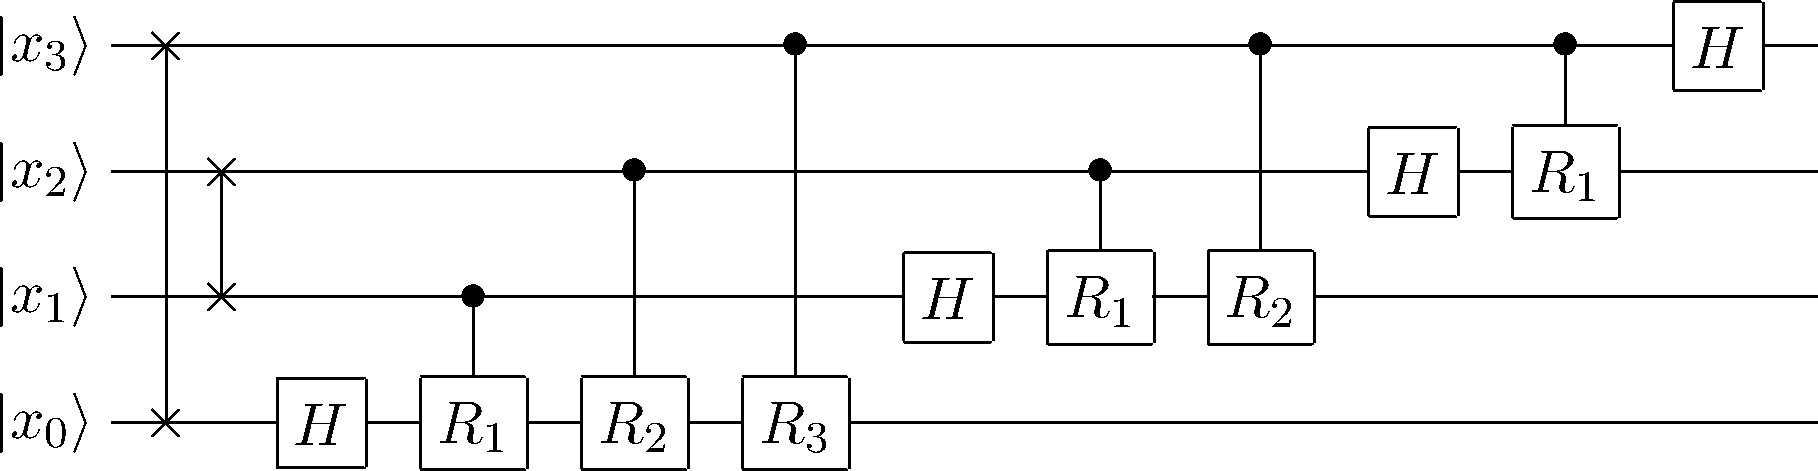
\includegraphics[width=0.8\textwidth]{qft}
    \caption{The circuit diagram for the quantum Fourier transform operation over 4 qubits}
\end{figure}

\paragraph{Implementation}
The implementation of the quantum Fourier transform in QIO is actually slightly different. By reversing the order of the controlled rotations, and the overall order of the gates, we can remove the need for SWAP operations at the start.
\begin{figure}[H]
    \centering
    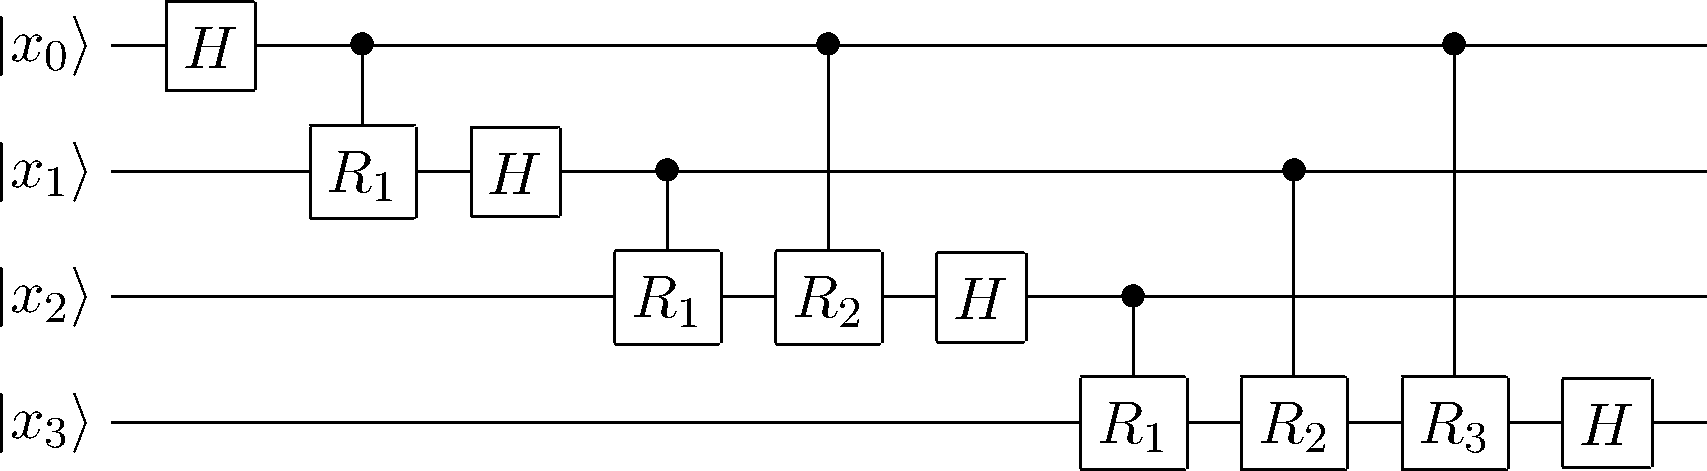
\includegraphics[width=0.8\textwidth]{qft2}
    \caption{The circuit diagram for an alternate quantum Fourier transform operation over 4 qubits}
\end{figure}

So, given a list of \texttt{Qbit}s, we need to apply a Hadamard gate, and then multiple rotation gates for each remaining \texttt{Qbit} in the list, where each gate is conditional on a distinct \texttt{Qbit}. I.e. given a list of 4 \texttt{Qbit}s, the unitary to construct is shown below, where \texttt{R k xn} is a $R_k$ gate on qubit $x_n$.
\begin{verbatim}
uhad x0 <> 
cond x0 (\x -> if x then R 1 x1 else mempty) <> uhad x1 <>
cond x1 (\x -> if x then R 1 x2) <> cond x0 (\x -> if x then R 2 x2) <> uhad x2 <>
cond x2 (\x -> if x then R 1 x3) <> cond x1 (\x -> if x then R 2 x3) <> 
cond x0 (\x -> if x then R 3 x3) <> uhad x3
\end{verbatim}

In order to create such a unitary operation, the implementation uses two recursive functions, \texttt{qftAcu} and \texttt{qftBase}. An entry function \texttt{qft} is then used to apply \texttt{qftAcu} over a list of \texttt{Qbit}s, using a new type class \texttt{Qdata a qa | a -> qa, qa -> a}.\par
This class defines what operations a quantum datatype must implement, and so relates heavily to the main structure of the \texttt{QIO} monad. \par
\begin{figure}[H]
    \centering
    \begin{minipage}[b]{0.54\textwidth}
        \begin{verbbox}
class Qdata a qa | a -> qa, qa -> a where
  mkQ :: a -> QIO qa
  measQ :: qa -> QIO a
  letU :: a -> (qa -> U) -> U
  condQ :: qa -> (a -> U) -> U
        \end{verbbox}
        \theverbbox
    \end{minipage}
     \begin{minipage}[b]{0.45\textwidth}
        \begin{verbbox}
instance Qdata Bool Qbit where
    mkQ = mkQbit
    measQ = measQbit
    letU b xu = ulet b xu
    condQ q br = cond q br
        \end{verbbox}
        \theverbbox
    \end{minipage}
\end{figure}

As you can see, we have already defined the operations for the relation between \texttt{Bool}s and \texttt{Qbit}s. The class is then used to define other quantum datatypes; pairs of datatypes, lists of datatypes, and most notably, a datatype relating \texttt{Int}s to quantum integers, \texttt{QInt}s.\par
Using two functions - one which creates a list of \texttt{Bool} values representing its \texttt{Int} argument, and the other which converts a list of \texttt{Bool} values to an integer - the datatype effectively works as an abstraction over a list of \texttt{Qbits} qs, stored as \texttt{QInt qs}.\par
The main operation used for the quantum Fourier transform is \texttt{condQ}. It  is used to perform conditional operations, such as the rotations described above, and enables the function \texttt{qft} to send its \texttt{[Qbit]} argument to \texttt{qftAcu} with the measured values of the qubits.\par
\begin{verbatim}
qft :: [Qbit] -> U
qft qs = condQ qs (\bs -> qftAcu qs bs [])
\end{verbatim}
From there, \texttt{qftAcu} deals with all the operations on a qubit, recursively moving from $x_0$ to $x_{n-1}$, while \texttt{qftBase} deals with each individual operation, i.e. the Hadamards and conditional Rotation gates.
\begin{verbatim}
qftAcu :: [Qbit] -> [Bool] -> [Bool] -> U
qftAcu [] [] _ = mempty
qftAcu (q:qs) (b:bs) cs = qftBase cs q `mappend` qftAcu qs bs (b:cs)

qftBase :: [Bool] -> Qbit -> U
qftBase bs q =  f' bs q 2
    where f' [] q _ = uhad q
          f' (b:bs) q x = if b then (rotK x q) `mappend` f' bs q (x+1)
                  else f' bs q (x+1)
\end{verbatim}

\subsubsection{Finding the period}
So, after applying the unitary $U_f$ to the state $\ket \phi _n \otimes \ket 0 _{n_0}$, and measuring the output register, the input register collapses to the state
$$\ket \Psi _n = \frac{1}{\sqrt m} \sum _{k=0}^{m-1} \ket{x_0 + kr}_n, \qquad  0 \leq x_0 < r, \qquad f(x_0) = f_0 $$
To extract the period $r$, we can apply the quantum Fourier transformation as shown below.
\begin{align*}
    U_{FT}\ket \Psi &= \frac{1}{2^{n/2}}\sum_{y=0}^{2^n-1}\frac{1}{\sqrt m}\sum_{k=0}^{m-1}e^{2\pi i(x_0 + kr)y/2^n} \ket y \\
    & = \sum_{y=0}^{2^n-1}e^{2\pi i x_0y/2^n} \frac{1}{\sqrt{2^nm}}\left(\sum_{k=0}^{m-1}e^{2\pi i kry/2^n}\right) \ket y
\end{align*}
The probability of getting the result $y$ is therefore given by
$$\frac{1}{2^nm}\left| \sum_{k=0}^{m-1}e^{2\pi i kry/2^n}\right|^2$$
which is highest when $y$ is close to integral multiples of $2^n/r$, giving the period as $r = 2^n / y$.

\subsubsection{The Implementation - an Alternative}
The quantum Fourier transformation has another use here; it's inverse can be used in a procedure known as phase estimation:

If we have a superposition of states
$$\frac{1}{2^{t/2}}\sum_{j=0}^{2^t-1}e^{2\pi i \varphi j} \ket j _n \ket u _m$$
we can apply the inverse quantum Fourier transform to get the state $\ket {\hat{\varphi}}_n \ket u _m$ where  $\hat{\varphi}$ is an approximation of $ \varphi $ up to $n$ bits. We can use this phase estimation procedure to execute Shor's algorithm.\par
To recap, after applying $U_f$, we are left with the state
$$\frac{1}{2^{n/2}} \sum_{x=0}^{2^n -1} \ket x \ket{b^x \Mod N}$$
Now, this state is approximately equal to 
$$\frac{1}{\sqrt{r}}\sum_{s=0}^{r-1}\left(\frac{1}{2^{n/2}} \sum_{x=0}^{2^n-1} e^{2\pi i x \frac{s}{r}} \ket x \ket{u_s}\right) \text{ where } \ket{u_s} = \frac{1}{\sqrt r} \sum_{k=0}^{r-1} e^{\frac{-2\pi isk}{r}} \ket{b^k \Mod N}$$
Applying the inverse quantum Fourier transform to this state gives
$$\frac{1}{\sqrt r}\sum_{s=0}^{r-1} \ket{( \frac{\hat s}{r} )} \ket{u_s}$$
and so measuring the first register will give us an integer result $\hat{\varphi} = \frac{\hat s}{r} \approx \frac{s}{r}$ up to $n$ bits. We can then use the continued fractions algorithm for $\frac{\varphi}{2^n}$ to calculate $r$.\par
On to the implementation. After getting a random integer coprime to $N$ - using a quantum random number generator defined in \texttt{QIORandom.hs} - the implementation applies Shor's algorithm with the function \texttt{shor :: Int -> Int -> QIO Int}, which initializes the qubits, applies hadamard gates to the first register, applies the function $b^x \Mod N$ and then applies the inverse of the quantum Fourier transformation. This is done efficiently using the already-defined quantum Fourier transformation, \texttt{qft}, and the function which reverses its unitary argument, \texttt{urev}. Finally, the first register is measured and its value returned as an \texttt{Int}. Due to the approximation and the small amount of qubits, this integer returned is approximately the period $r$.\par
All that is left is to check if $r$ is even and not equal to $0$, and that $x-1 \neq 0 \Mod N$. If all these are true, $N$ is factorized using \texttt{gcd (x-1) n} and \texttt{gcd (x+1) n}.


\section{Quantum Circuit Builder}
\subsection{Analysis}
As mentioned earlier, the quantum circuit builder will be similar to the IBM Q Composer \cite{ibmqexperience}. Emphasis needs to be placed on usability, giving users a stable, reliable and most notably, easy to use graphical platform they can use to create and simulate quantum computations on a classical computer using Haskell and the QIO package.\par
Therefore, the user should be presented with a readable and intuitive circuit diagram; minimal in design to avoid confusion while also being large enough to convey the details of the circuit. The user needs to be able to alter the amount of qubits on the circuit. Quantum gates will be able to be moved on/off the circuit, enabling easy creation of a new quantum circuit without confusion. Buttons need to be available to run or simulate the created circuit, presenting the results of either to the user in a clear manner. The circuit needs to be able to be edited, allowing the moving of gates off the circuit, and changing the order in which they appear. Gates also need to be able to be made conditional to other specified qubits so that more complex quantum circuits can be built.

\subsubsection{Specification}
\paragraph{Functional}
\begin{enumerate}
        \item A graphical interface will be presented to the user in its own window upon running the program. Closing this window will end the program entirely.
        \item An initial circuit will be shown containing three qubits, initially in the state $\ket 0$.
        \item Buttons will be available to add or remove qubits from the circuit, and all qubits will initially be in the state $\ket 0$.
        \item Quantum gates will be able to be moved on and off the circuit using a mouse.
        \item While picked up, gates must be able to be removed, allowing the user to cancel their original intention.
        \item Gates will be able to be made conditional on other qubits, which also need to be specified before placement.
        \item Gates must be able to be moved around the circuit, while maintaining the layout of the other gates on the circuit.
        \item Buttons can be used to run or simulate the circuit, using the appropriate \texttt{run} and \texttt{sim} functions. The results of these functions then need to be presented to the user clearly.
\end{enumerate}

\paragraph{Non-functional}
\begin{enumerate}
    \item \textbf{Usability} Emphasis must be placed on usability. All aspects of the graphical interface must be large enough to read and interact with, while also being clear on their intended use. A user guide will need to be created, explaining in appropriate detail each part of the program, and explain appropriate use cases.
    \item \textbf{Reliability} The program must be able to be run at any time on any appropriate computer with a Haskell compiler installed. It must not crash at any point, and so should only execute simple functions to present and allow interaction with the interface. However, the running and simulating of circuits will rely on QIO's functions, which are already relatively reliable.
    \item \textbf{Performance} Due to its graphical nature, the interface needs to be efficient in its rendering and interaction functions in order to minimise user frustration and confusion.
    \item \textbf{Quality} The functional and non-functional specifications here needs to be met as best as possible to maximise the program's quality. It must be thoroughly tested with both simple and complex quantum circuits to ensure it is robust and can handle the user's needs.
    \item \textbf{Documentation} As mentioned above, a user guide will need to be created to provide instruction to the user on how to interact with the program. Simple explanation needs to be provided on what each aspect of the interface does, alongside the detailing of common use cases of the program.
\end{enumerate}

\subsection{Graphics in Haskell}
As the circuit builder will be created in Haskell, a suitable graphics package must be used to deal with rendering as well as user interaction. Therefore, research is first done to find the most appropriate package to ensure program quality alongside an understandable implementation.

\subsubsection{Diagrams}
Diagrams \cite{diagrams} is ``a powerful, flexible, declarative domain-specific language for creating vector graphics, using the Haskell programming language.'' It's core library aims to be as simple and flexible as possible, built using a small set of primitive types and operations. The main page of the package \cite{diagrams} provides access to a quick start tutorial, giving basic instruction on installation and simple use, along with a full user manual explaining each aspect of the package, and how to create complex images. \par
Drawing both simple and complicated images is very easy with this library. For example, to draw a circle of radius 1 is done quickly by executing \texttt{circle 1}. Shapes can be combined using functions such as \texttt{atop}, or placed side-by-side with the operators \texttt{|||} and \texttt{===} for horizontal and vertical placement respectively. Diagram attributes, such as line width and fill colour, are defined using simple functions taking in the value to set the attribute to, such as \texttt{lw veryThick} and \texttt{fc red}. Diagrams can also be transformed using \texttt{scale}, \texttt{rotate} and \texttt{reflect} functions. The diagrams form a monoid under \texttt{atop} as well, and so two diagrams can be superimposed using the mappend operator \texttt{<>} instead of \texttt{atop}. Other things, such as transformations and paths, also form monoids allowing easy construction of complex images.\par
While this package does seem promising, it is not suitable for creating a quantum circuit builder. The simple and effective commands would be extremely useful for rendering purposes, however the program does not need complex shapes to be drawn. The diagrams package also draws to files, such as .svg files using its SVG backend, which is the opposite of what is required by the circuit builder. User interaction is also not supported, reinforcing the idea that this package is not suitable for use in this case. 

\subsubsection{Gloss}
Gloss \cite{gloss} ``hides the pain of drawing simple vector graphics behind a nice data type and a few display functions''. The package abstracts the use of OpenGL and GLUT, promising that you can ``get something cool on the screen in under 10 minutes.'' Much like diagrams, it aims to be as simple as possible while also being flexible, allowing simple and complex images to be drawn effectively. Learning the package is not quite as easy to do as with diagrams, as there is no quick start tutorial or user guide. Instruction is instead given using straightforward examples, ranging from drawing simple text on the screen to animating the movement of complex images over a background. Luckily, the package is intuitively designed, and so being able to create images, interact with the user and draw animations, can be learnt with the use of these examples and reading through some of the code.\par
Much like with the diagrams package, shapes can be drawn extremely easily using functions like \texttt{rectangleSolid} and \texttt{thickCircle}. Text can also be drawn using a simple function \texttt{text} which takes in the \texttt{String} to draw. Everything that can be drawn is defined under a \texttt{Picture} data type, and attributes of shapes can be changed by functions of the type \texttt{Picture -> Picture}. This means such functions can be combined with the \$ character. For example, creating a solid red circle with radius 5 at coordinates (100,100) is done with the line \texttt{translate 100 100 \$ color red \$ circle 5}. Pictures can be combined and altered as one using the \texttt{pictures :: [Picture] -> Picture} function.\par
The \texttt{main :: IO ()} function is used as the entry point to programs using gloss, which provides multiple functions for different use cases. For example, the \texttt{display :: Display -> Color -> Picture -> IO ()} function draws the \texttt{Picture} on a display specified by the \texttt{Display} type with a background colour specified by the \texttt{Color} type. The main function here though is the function \texttt{play}.
\begin{verbatim}
 play :: Display -> Color -> Int 
         -> world -> (world -> Picture) -> (Event -> world -> world) 
         -> (Float -> world -> world) -> IO ()
\end{verbatim}
This function presents a display specified with a given background colour and a framerate. It then uses a function of type \texttt{(world -> Picture)} to render a world, starting with the intial world specified, and allows user interaction with a function of type \texttt{(Event -> world -> world)}. The final argument is then used to step the world by one frame, allowing animations to be created.\par
This package is a great fit for use in creating a graphical quantum circuit builder. The simple functions provided to draw basic shapes, which can be extended to draw more complex objects, work perfectly, and the availability of a function to draw text given a string would come in handy. The abstraction of user interaction with an \texttt{Event} type is great to create simple yet effective functions which handle all necessary types of user interaction. However, the lack of even a small quick start guide means the, albeit basic, knowledge required to use the package has to be learnt through limited examples, code reading and trial and error.

\subsubsection{The Package of Choice}
The most appropriate package for use in creating the quantum circuit builder is gloss. The simple abstraction to OpenGL and GLUT means drawing shapes is easily done, effective and efficient. The \texttt{play} function means handling of user interaction can be done with one simple function, and is made to be used with one world type in mind. This would enable the implementation to be built around a circuit record, storing the amount of qubits on the circuit, the gates on the circuit etc.\par
The \texttt{pictures} function will allow transformations to be performed on groups of images, such as all the buttons or the rows of qubits, making the implementation simple and easy to understand for others. Rendering of text will be used frequently to intuitively describe buttons and present results of computation to the user. 

\subsection{Implementation}
\subsubsection{The Window}
To start off, the implementation requires a \texttt{main :: IO ()} function to display a window to the user, and provide the necessary functions to the \texttt{play} function mentioned above. The window will have the title ``Circuit'', with a width of 1024 and height of 720, placed initially at the position (10,10) on the screen. 
\begin{verbatim}
window :: Display
window = InWindow "Circuit" (floor width, floor height) (10,10)

main :: IO ()
main = play window
            white
            30
            initialCircuit
            draw
            handleEvent
            (const id)
\end{verbatim}
This will produce a window described above, with a white background colour and an fps of 30. Given an initial circuit, it will draw using the \texttt{draw} function and handle user interaction via \texttt{handleEvent}. Finally, as animations are not necessary, the last function simply just returns whatever it is given.\par
Each aspect of the program, specifically the \texttt{main} function, the circuit, the rendering and the interaction will be located in its own file, ensuring simple modularity. 

\subsubsection{The Circuit}
As explained above, gloss relies upon a single data type to store all the details of the ``world'', or in this case, the circuit. Therefore, the implementation requires a data type \texttt{Circuit}, which will be a record containing all the circuit details, including the qubits in the circuit and the gates, and their locations, on the circuit.
\begin{verbatim}
data Circuit = Circuit { qubits :: [Int],
                         gates :: [Gate]
                       } deriving (Eq, Show)

initialCircuit :: Circuit
initialCircuit = Circuit { qubits = [0..2],
                           gates = [] }
                       
data Gate = Null,
          | Had Int [Int]
          | PX Int [Int]
          | PY Int [Int]
          | PZ Int [Int]
          | Swap Int [Int]
          deriving (Eq, Show)
          
instance Ord Gate where
  compare g1 g2 = compare (getCol g1) (getCol g2)
\end{verbatim}
A datatype \texttt{Gate} is also created, restricting a Gate to be of a specific type, with a column \texttt{Int} and a list of \texttt{Int}s representing the qubits it operates on, where the gate is applied to the last qubit in the list conditional on the first $n-1$ qubits before. If only one qubit is in the list, it is not conditional and acts as a standard gate. The only exception here is the SWAP gate, which will only be able to have a list of two qubits and will not be conditional. Gates will also be able to be sorted by their column, allowing easy sorting over lists of gates.

\subsubsection{Rendering}
The \texttt{draw} function is the main entry point in rendering the interface, and takes in a \texttt{Circuit} to draw. Every button and gate on the interface will look the same; a simple square white box, with a black outline and a symbol inside indicating what it does. For example, the button representing the Hadamard gate will need to have a ``H'' inside of it. So, first off, its easiest to define a function \texttt{drawBox} which will be used to draw the square box at the position passed in. The coordinates of each item will also be fashioned into a grid, so that the rows and columns on the circuit line up smoothly, with equal spacing between everything. For this, we can use two functions, \texttt{calcX} and \texttt{calcY} along with a \texttt{spacing Float} constant defined at the start.
\begin{verbatim}
drawBox :: Int -> Int -> String -> Picture
drawBox c q t = translate (calcX c) (calcY q) $
                pictures [ color white $ rectangleSolid (spacing/2) (spacing/2),
                           color black $ rectangleWire (spacing/2) (spacing/2),
                           color black $ translate (-spacing/8) (-spacing/8) 
                               $ scale 0.1 0.1 $ text t ]
\end{verbatim}

\begin{wrapfigure}{l}{0.15\textwidth}
    \centering
    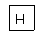
\includegraphics[width=0.1\textwidth]{drawbox1}
    \caption{The result of drawBox 0 0 ``H''}
\end{wrapfigure}

As can be seen to the left, the box is drawn as required however the text is still off even after moving it, and even then still looks out of place. The lines making up the ``H'' are not big enough, and are not aesthetically pleasing. Therefore, a function \texttt{drawText} is required to handle drawing text onto the buttons.\par
This function will take in a \texttt{String}, such as ``H'', and draw it using the appropriate rectangles. As the program will only be required to draw certain symbols, pattern matching can be used to handle all specific cases, and then return a blank picture for any unsupported symbol.\par
From here, all of the buttons can be drawn efficiently using a list containing the text for each button, and mapping over this list with increasing values of x to draw each button. For this, a special case of \texttt{drawBox} needs to be implemented which does not translate the drawn picture to an x and y, allowing this to be handled by the calling function. Finally, a thicker line needs to be drawn under the buttons dictating a separation from the buttons and the circuit. However, as thick lines are not possible in gloss, the program simply draws two lines, with one under the other.
\begin{figure}[H]
    \centering
    \begin{minipage}{0.25\textwidth}
        \begin{verbatim}
buttons :: [String]
buttons = [ "+",
            "-",
            "H",
            "X",
            "Y",
            "Z",
            "Swap",
            "Run",
            "Sim",
            "Clear" ]
        \end{verbatim}
    \end{minipage}
     \begin{minipage}{0.7\textwidth}
        \begin{verbatim}
drawButtons :: Picture
drawButtons = pictures $
              (map (\(x, b) -> translate (x*spacing) 0 $ 
                  drawBox (-1) (-1) b) $ zip [0..] buttons) ++
              [ color black $ line [(-spacing/2, -spacing/2), 
                                    (width-spacing, -spacing/2)],
                color black $ line [(-spacing/2, -spacing/2-1), 
                                    (width-spacing, -spacing/2-1)],
                color black $ line [(3*spacing/2, spacing/3), 
                                    (3*spacing/2, -spacing/3)],
                color black $ line [(13*spacing/2, spacing/3), 
                                    (13*spacing/2, -spacing/3)]]
        \end{verbatim}
    \end{minipage}
\end{figure}

\begin{wrapfigure}{r}{0.47\textwidth}
    \centering
    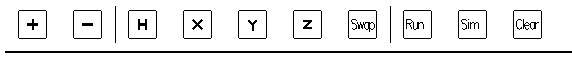
\includegraphics[width=0.45\textwidth]{buttons1}
    \caption{The result of drawButtons}
\end{wrapfigure}
The circuit now needs to be rendered. Given a \texttt{Circuit}, functions are required to draw the qubits and the gates. The qubits are simply black lines with the text ``|0>'' in front to show that they are initially in the $\ket 0$ state. It will also show the number of the qubit, improving the readability of the circuit. All this is done by mapping the drawing of the qubit over the qubit list in the circuit record passed in.\par
Drawing the gates is slightly more complicated. Due to the design of the \texttt{Gate} type, each gate needs to be handled individually. However, each gate is handled pretty much the same, with the only difference being the Controlled-X gate (i.e. when the Pauli-X gate has multiple qubits in its list) and the SWAP gate.\par
The function \texttt{drawGate} will take in a gate with a column value \texttt{c} and the qubits it acts on given by \texttt{qs}. Black dots representing the conditionality are drawn for each $n-1$ qubit in the list, and a line is then drawn connecting them to the last qubit. Finally, a box is drawn on the last qubit, with a symbol pertaining to the type of gate. The only complication here is when the conditional qubits in the list are both above and below the last qubit. In order to deal with this, a line has to be drawn between each qubit individually, instead of one long line from the first qubit to the last.\par
In order to draw a Controlled-X gate, the conditional qubits are dealt with in a similar fashion, however instead of a box containing an ``X'' on the last qubit, a circle will be drawn with a plus inside; the same as shown in section 1.6.2. Finally, drawing the SWAP gate is simply a case of drawing a cross on each qubit in the list, with a vertical line connecting them together.\par
Combining all this into one function \texttt{drawCircuit circuit = pictures [ drawQubits (qubits circuit), drawGates (gates circuit)]} produces the expected result over an initial circuit with gates already included.
\begin{figure}[H]
    \centering
    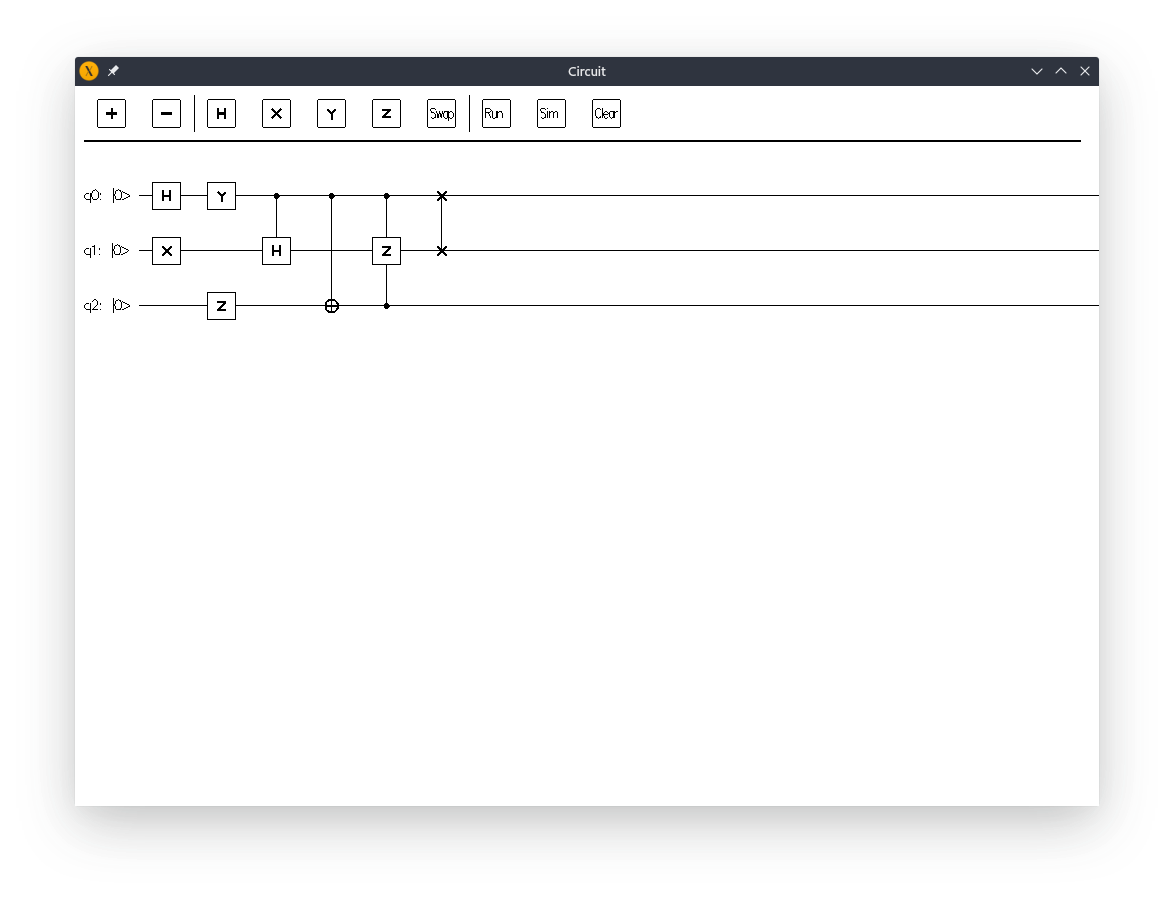
\includegraphics[width=0.8\textwidth]{examplecircuit}
    \caption{The result of drawing over a circuit with three qubits and gates = [Had 0 [0], PX 0 [1], PY 1 [0], PZ 1 [2], Had 2 [0, 1], PX 3 [0, 2], PZ 4 [0, 2, 1], Swap 5 [0, 1]]}
\end{figure}

\subsubsection{User Interaction}
Handling user interaction is done via the \texttt{handleEvent} function. This function takes in an \texttt{Event} and a \texttt{Circuit}, and then returns a \texttt{Circuit} which it has altered in some way. Therefore, we can't directly call rendering functions, and instead need a way of storing user interaction details in the \texttt{Circuit} type. Simply adding an \texttt{edit :: String} and \texttt{mouse :: (Float, Float)} will achieve this. \texttt{Edit} will store the gate picked up at that moment, i.e. ``H'' for a Hadamard gate, while \texttt{mouse} will store the location of the mouse, allowing the picked-up gate to be seen following the mouse and knowing its location when dropped.\par
The \texttt{Event} type contains all the details of a user event, such as a key press or mouse movement. It can take one of three distinct types:
\begin{verbatim}
data Event = EventKey Key KeyState Modifiers (Float, Float)
           | EventMotion (Float, Float)
           | EventResize (Int, Int)
\end{verbatim}
The \texttt{Key} type will contain either the character of the key pressed, the special key pressed (e.g. the Enter key) or the mouse button pressed (e.g. the left mouse button). The \texttt{KeyState} dictates if the key has been pressed or released, while the \texttt{Modifiers} represent whether the ctrl, shift or alt keys are also down. The \texttt{(Float, Float)} in both \texttt{EventKey} and \texttt{EventMotion} contain the current x and y positions of the mouse in the window. \par
Upon pressing the left mouse button down, the user may want to either click on a button, click on a location on the circuit to place down a picked-up gate, or click on a gate already on the circuit to pick it up. Using a function \texttt{mousePosition :: (Float, Float) -> Circuit -> Circuit}, the program can check which of these has occured. If the right mouse button is instead pressed, any picked up gate is cleared, allowing the user to easily clear gates from the circuit or stop placing a gate down when one is picked up.\par
\paragraph{Button Press}
Using the \texttt{buttons} list created earlier, the button clicked can be retrieved by finding the column on the grid described earlier which the mouse is inside. If the mouse is indeed over a button, a function \texttt{buttonPress :: Circuit -> String -> Circuit} is called to handle which button was pressed. If the \texttt{String} passed in is a ``+'' or a ``-'', then a qubit needs to be added or removed from the circuit. If the \texttt{String} is ``Clear'', then all gates need to be removed from the circuit. The ``run'' and ``sim'' cases will be handled later on. In any other case, the \texttt{edit} record in the \texttt{circuit} needs to be updated to reflect that a gate has been selected from the buttons.\par
Adding a qubit is simply a case of appending \texttt{[length \$ qubits circuit]} to the end of the qubits in the circuit, and removing a qubit is done by applying \texttt{init} to the list of qubits as long as the list is not empty. However, at the same time, all the gates on this qubit must also be removed, including gates conditional on the qubit. In order to do this, a function \texttt{getQs :: Gate -> [Int]} is used to extract the list of qubits from a gate, and a check is then done to see if the qubit to remove is included in this list. If so, the gate needs to be removed, else nothing is done. All this, combined into a function \texttt{remGateOnQubit :: Int -> Gate -> Gate}, is then mapped over the list of gates in the circuit, removing them as necessary. The removal is actually done by setting the gate to \texttt{Null} if it needs to be removed, and then applying \texttt{filter (/= Null)} over the returned list.\par
If the Clear button is instead clicked, we simply set the \texttt{gates} record in the \texttt{circuit} to be \texttt{[]}. If a gate button is pressed, the \texttt{edit} record in the \texttt{circuit} is set to the \texttt{String} representing the gate. After this, the rendering functions need to be changed to show that a gate has been picked up.\par
\begin{wrapfigure}{l}{0.5\textwidth}
    \centering
    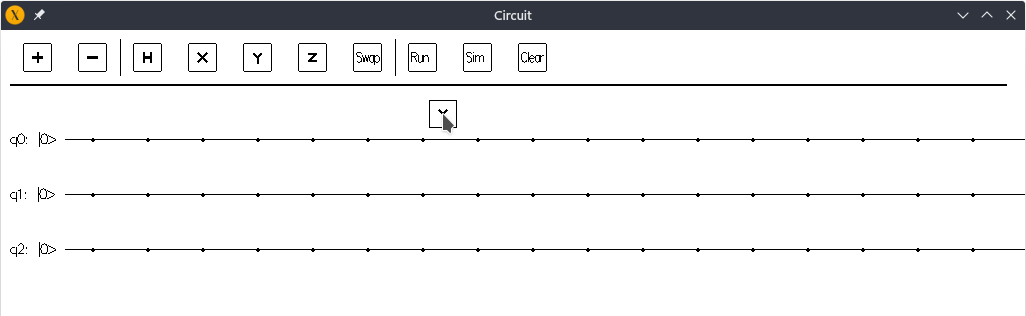
\includegraphics[width=0.48\textwidth]{pickupgate}
    \caption{A picked up Pauli-Y gate over an empty circuit.}
\end{wrapfigure}

In the \texttt{draw} function described earlier, dots must be drawn on all empty sections of the circuit to highlight that a gate can be placed here. This is done by drawing a black circle at the calculated x and y location on the circuit, and then mapping this over all the qubits on the circuit and a list of \texttt{[0..20]}, as roughly 20 columns fit in the window. Following this, the gate selected needs to be drawn under the mouse cursor by translate the result of the \texttt{drawBox} function to the mouse coordinates stored in the \texttt{mouse} record of the \texttt{circuit}.

\paragraph{Placing a Gate}
If the \texttt{edit} record in the \texttt{circuit} already has a value, then a gate has already been picked up. Therefore, if the mouse is over the circuit, then the user wants to place the gate down. The function must then calculate the column and row that it is being placed onto and pass it into a function \texttt{addGate :: Int -> Int -> Circuit -> Circuit}.\par
Three things can then occur: the position on the circuit is already taken, the mouse is between two columns, or the position is empty. Dealing with the case of the position being taken is easiest, and just requires nothing to be changed; the gate is still picked up and the circuit is not altered. \par
If the position is empty, the only thing required to do is to add a new gate to the circuit's list, with the column and row calculated earlier and the type specified by the \texttt{edit} record. Then, the \texttt{edit} record is cleared to show the gate has been placed down.\par
If the mouse is between two columns, the user wants to effectively add a new column in between, and place the gate there. Therefore, all the gates with a column value higher than or equal to the position need to be moved right by one column. As there is an instance of \texttt{Ord} defined for gates already, the \texttt{sort} function can be used to sort by increasing column order. Following this, the \texttt{span} function can be used along with a new function \texttt{lteCol :: Int -> Gate -> Bool} - which returns True when the gate passed in is in a column less than or equal to the column passed in - the list of gates can be split up into the form \texttt{(bG, aG)}, where \texttt{bG} contains the gates before the new column and \texttt{aG} contains the gates which will be after the new column (i.e. the column value of each gate in this list needs to also be incremented by one). Then, the new gate can be placed in between the two sets, creating a new column for it to be placed onto. \par

\paragraph{Picking up a Gate}
Finally, if the \texttt{edit} record is empty and the mouse is over the circuit, the user wants to pick up a gate from the circuit. In this case, the function calculates the column and row it is being picked up from and passes it into a function \texttt{pickUpGate :: Int -> Int -> Circuit -> Circuit}. This function then calculates whether or not the mouse is in fact over a gate on the circuit, and if it is the gate is deleted (note that the column is not deleted if there is nothing else in it) and then the \texttt{edit} record is changed to show the gate has been picked up.\par

\paragraph{Key Press}
The number keys will be used to specify the control qubits for a gate which is picked up. For example, while a Hadamard gate is picked up, pressing the '0' key will specify that this gate will be conditional on the qubit ``q0''. Handling this is relatively simple using the \texttt{EventKey (Char c) ...} form of the \texttt{Event} type.\par
If \texttt{c} is a number key, then the \texttt{edit} record of the \texttt{circuit} is updated by appending the a space along with the number pressed as long as a gate is picked up. If the gate is a SWAP gate, then this can only occur once (as the key pressed represents the qubit to swap with when placed on a different qubit), and so the length of the \texttt{edit} record must be checked. If the backspace key is instead pressed, causing \texttt{c} to equal \texttt{'\textbackslash b'}, then the conditional qubits need to be cleared, reverting the \texttt{edit} record back to simply store the gate type picked up.\par
\begin{verbatim}
handleEvent (EventKey (Char c) Up _ pos) circuit =
  case head e of
    'H' | c == '\b'                             -> circuit { edit = "H" }
    'H' | c >= '0' && c <= '9'                  -> circuit { edit = e ++ [' ', c] }
    ...
    'S' | c >= '0' && c <= '9' && length e == 4 -> circuit { edit = e ++ [' ', c] }
    ...
  where
      e = edit circuit
\end{verbatim}
\begin{wrapfigure}{r}{0.45\textwidth}
    \centering
    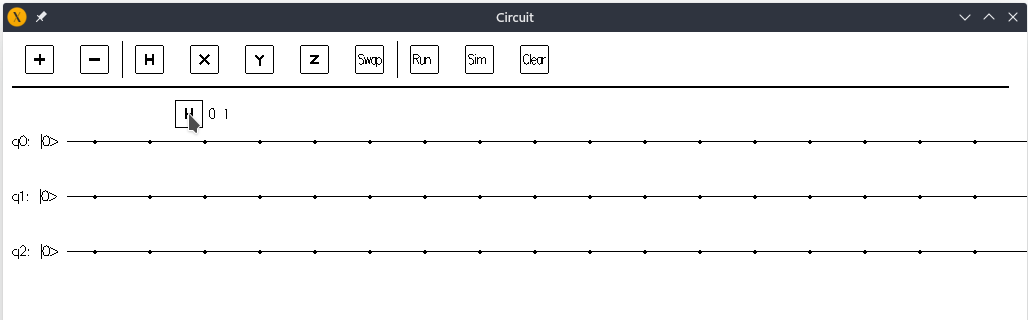
\includegraphics[width=0.43\textwidth]{editH}
    \caption{Picking up a Hadamard gate, with control qubits ``q0'' and ``q1''.}
\end{wrapfigure}

During the render process, the numbers already pressed can be shown easily using gloss' \texttt{text} function. The implementation must now be able to handle placing gates down with conditional qubits. In order to acheive this, a function \texttt{getControls :: String -> [Int]} is created. This function removes all spaces from the \texttt{String} passed in, removes duplicate numbers, and then converts each character into its relevant \texttt{Int} using the \texttt{read} function. Now, new gates can be created by appending the qubit it is placed on at the end of the list of control qubits. If any of the control qubits are equal to the qubit the gate is being placed on, the operation is cancelled to prevent errors from occuring.\par 

\subsubsection{Executing the Circuit}
In order to execute the circuit, it first needs to be compiled. This is actually fairly simple to do using the list of qubits and list of gates in the circuit. Each qubit in the list needs to be created in the state $\ket 0$, and then the unitary operation relating to the circuit needs to be executed using the \texttt{applyU} function, and finally the qubits are measured.\par
\begin{verbatim}
compileCircuit :: Circuit -> QIO [Bool]
compileCircuit circuit = do
  qs <- mkQbits (length $ qubits circuit) False
  applyU (gatesToU (gates circuit) qs)
  measQbits qs
\end{verbatim}
The \texttt{gatesToU} function is used to recursively convert each gate into its corresponding unitary operation, using the function \texttt{gateToU :: Gate -> [Qbit] -> U}, and then combine the operations using the \texttt{<>} operator. Upon being given a gate, the \texttt{gateToU} function will map the relevant unitary operation (e.g. \texttt{uhad} for a Hadamard gate) over the list of qubits, where each qubit is at the index specified by the gate's qubit list. A function \texttt{condU} is used to conditionally apply the operation according to the first $n-1$ qubits in the gate's qubit list.\par
When the circuit is compiled, it will be able to be run or simulated using the appropriate functions when the user clicks either the ``Run'' or ``Sim'' buttons described above. The result of either is then saved in a new record \texttt{result :: String} inside the \texttt{circuit} type. For simulation, this is done simply using \texttt{show \$ sim \$ compileCircuit circuit}, as the result of \texttt{sim} can be converted straight into a \texttt{String}. However, running the circuit is more difficult, as \texttt{run} returns the type \texttt{IO a}, in this case \texttt{IO [Bool]}.\par
As an \texttt{IO a} type cannot be converted into a \texttt{String}, as it is wrapped in the \texttt{IO} monad, we must find a way of extracting the values. This can be done using the function \texttt{unsafePerformIO :: IO a -> a}, which does what we want by performing the IO actions as a pure function. Because of this, Haskell will optimize the actions (as it does not realise it is an IO action) and so certain side-effects may not be executed. However, the computation will not produce any side-effects, and its only action is to generate a random number using \texttt{Random.randomRIO}, and so it is safe to use in this instance, producing a \texttt{String} result via \texttt{show \$ unsafePerformIO \$ run \$ compileCircuit circuit}.\par
In order to render the results, the \texttt{draw} function needs to be altered. The \texttt{result} record in the \texttt{circuit} will contain a \texttt{String} of what to draw, and so gloss' \texttt{text} function can be used to render the text underneath the rows of qubits. \par
The execution of the built circuit can be made easier changing the \texttt{handleEvent} function, so that when the Enter key is pressed, the circuit is run.
\begin{figure}[H]
    \centering
    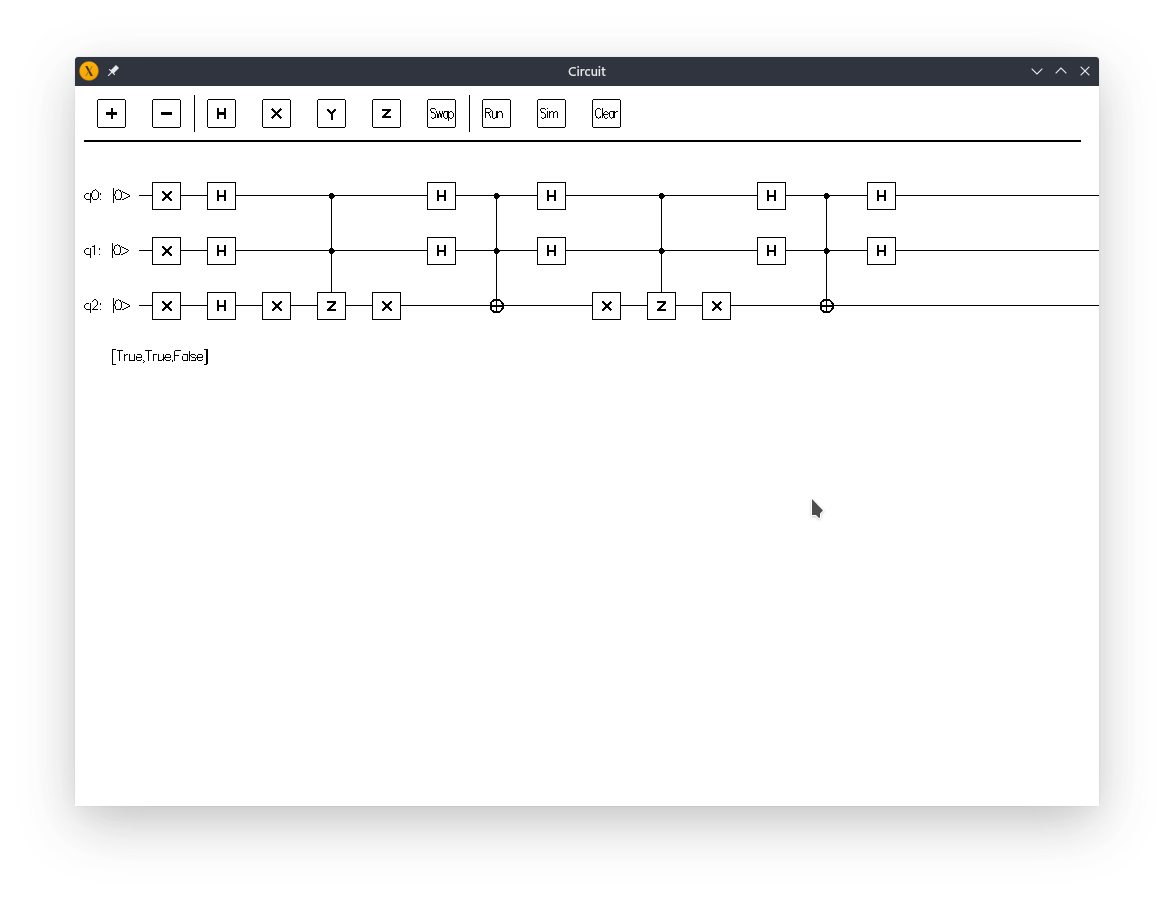
\includegraphics[width=0.8\textwidth]{rungrover}
    \caption{Running Grover's algorithm, searching for the state $\ket{110}$, over three qubits.}
\end{figure}



\subsection{Testing}


\section{Reflections}

\newpage
\bibliographystyle{alpha}
\bibliography{diss}

\end{document}
